\chapter{Extracción de puntos característicos}
\label{capitulo3}
\lhead{Capítulo 3. \emph{Extracción de puntos característicos}}


\section{Introducción}

En el capítulo anterior se valuaron los distintos tipos de técnicas de establecer la relación para el registro de imágenes, y en base a estos se planteó el uso de características locales para establecer la correspondencia entre imágenes. En el presente capitulo se pretende explicar en detalle el funcionamiento de los algoritmos de detección mas usados en estas aplicaciones, así como también la importancia de los avances que cada uno introduce. Después se presentan los algoritmo de emparejamiento, así como también una explicación de su funcionamiento. Finalmente, con el objetivo de caracterizar cada uno de los detectores y emparejadores, se implementa un módulo para comparar el rendimiento de estos bajo distintas condiciones. Esto nos permitirá luego seleccionar el mejor algoritmo para cada aplicación.

\section{Revisión teórica}

\subsection{Detectores y descriptores de características}

Antes mencionar la evolución de los algoritmos de detección de puntos de interés, primero es necesario definir que son estos. Los puntos de interés, puntos clave, o \textit{"features"} (en español: características) como son comúnmente llamados, son regiones en una imagen que contienen patrones específicos, lo que hace que puedan ser fácilmente seguidos o ubicados en otra imagen. Tuytelaars y Mikolajczyk \cite{Tuytelaars} definen un punto característico local como \textit{``un patrón en la imagen que difiere de su vecindario directo''}. De esta forma, se considera que los puntos característicos deben proporcionar la posibilidad de ser identificados en diferentes imágenes con el objetivo de emparejarlos.

Para alcanzar este objetivo los detectores y extractores de puntos característicos deben cumplir con ciertas propiedades que les permita funcionar bajo distintas condiciones, en concreto se busca que estos algoritmos cumplan con las siguientes propiedades:

\begin{itemize}
	\item \textbf{Robustez:} El algoritmo debe ser capaz de detectar la misma ubicación del punto característico independientemente ante cambios en la escala, rotación, traslación, iluminación, transformaciones geométricas, artefactos de compresión y ruido.
	
	\item \textbf{Repetibilidad:} El algoritmo debe ser capaz de detectar el mismo punto característico de la misma escena bajo cambios en el punto de vista.
	
	\item \textbf{Exactitud:} El detector debe localizar el punto característico de manera precisa (misma ubicación de píxel). Especialmente para tareas de alineación de imágenes.
	
	\item \textbf{Generalidad:} El algoritmo debe ser capaz de detectar puntos que pueden ser usadas en distintas aplicaciones, es decir, que detecte varios tipos de características (esquinas, burbujas, etc.)
	
	\item \textbf{Eficiencia:} El algoritmo debe ser capaz de detectar puntos característicos en nuevas imágenes a gran velocidad, para soportar aplicaciones en tiempo real.
	
	\item \textbf{Cantidad:} El algoritmo debe detectar todos, o casi todos los puntos característicos presentes en la imagen. 
	
\end{itemize}



\begin{figure}[H]
	\centering
	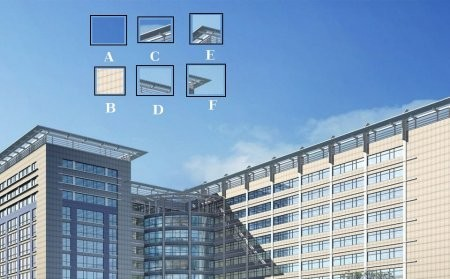
\includegraphics[width=0.7\textwidth]{features}
	\caption[Caracterización de regiones en una imagen]{Caracterización de regiones en una imagen\protect\footnotemark}
	\label{imagen:features}
\end{figure}
\footnotetext{\url{https://docs.opencv.org/3.0-beta/doc/py_tutorials/py_feature2d/py_features_meaning/py_features_meaning.html}}
%https://docs.opencv.org/3.0-beta/doc/py_tutorials/py_feature2d/py_features_meaning/py_features_meaning.html

Llegados a este punto es necesario definir el funcionamiento de los algoritmos detectores, y que consideran estos como puntos característicos, basados en la definición previamente planteada. Atendiendo a la imagen \ref{imagen:features}, se puede observar que se caracterizan seis áreas de interés. Analizando estos segmentos, vemos que \textbf{\textit{A}} y \textbf{\textit{B}} corresponden con superficies planas, lo que hace que sea muy difícil identificar la ubicación exacta de estas superficies en la imagen original. Por otro lado, tenemos las regiones \textbf{\textit{C}} y \textbf{\textit{D}}, las cuales corresponden con bordes en la imagen, si bien, se puede limitar en gran medida el área de búsqueda hacia toda las regiones del mismo bordes, sigue siendo difícil acertar con la ubicación correcta. Por ultimo, analizando las regiones \textbf{\textit{E}} y \textbf{\textit{F}} tenemos que corresponden a esquinas de la imagen original, en este caso se puede identificar fácilmente la ubicación exacta de la región en la imagen.

A partir de esta idea, en la cual se consideran las esquinas como regiones fácilmente identificables en una imagen, en \textit{1988} nace el primer algoritmo de detección de puntos de interés llamado Detector de esquinas de Harris \cite{harris} (nombre original en inglés: Harris Corner Detector), y como su nombre lo indica está basado en la detección de esquinas.

Retomando el concepto planteado previamente, este detector busca la diferencia de intensidad de una región con su entorno directo, es decir, se detectará una esquina para aquellas regiones que presenten una alta variación de intensidad, al desplazar la ventana estudiada en cualquier dirección. En la figura \ref{imagen:harris-window} se puede apreciar visualmente como funciona esta ventana de búsqueda.

\begin{figure}[H]
	\centering
	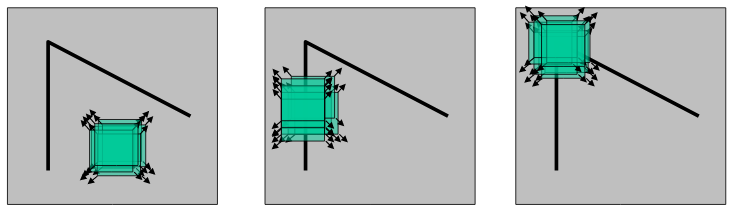
\includegraphics[width=0.9\textwidth]{harris-window}
	\caption[Ventana de búsqueda para de detección de esquinas]{Ventana de búsqueda para de detección de esquinas, adaptado de\protect\footnotemark}
	\label{imagen:harris-window}
\end{figure}
\footnotetext{\url{https://dsp.stackexchange.com/questions/14338/}}
%https://dsp.stackexchange.com/questions/14338/

Cuando se trabajan con detectores de características, se desea que estos sean invariantes ante la mayor cantidad de variables posibles, tal y como se menciona en la propiedad de robustez que deben tener estos algoritmos. Si bien el detector presentado anteriormente es invariante ante la traslación y la rotación (ya que las esquinas se mantienen como esquinas si son rotadas o desplazadas), no funciona de la misma forma ante cambios de escala. Como se observa en la figura \ref{imagen:corner-scale}, una región considerada como esquina, se podría considerar plana si es ampliada.

\begin{figure}[H]
	\centering
	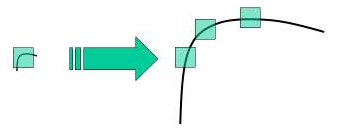
\includegraphics[width=0.85\textwidth]{corner-scale}
	\caption[Efecto del escalado sobre las esquinas]{Efecto del escalado sobre las esquinas	\protect\footnotemark}
	\label{imagen:corner-scale}
\end{figure}
\footnotetext{\url{https://docs.opencv.org/3.0-beta/doc/py_tutorials/py_feature2d/py_sift_intro/py_sift_intro.html}}
%https://docs.opencv.org/3.0-beta/doc/py_tutorials/py_feature2d/py_sift_intro/py_sift_intro.html

Con el fin de conseguir detectar los mismos puntos ante cambios en la escala de la imagen, Lindeberg, T. \cite{log} propone un algoritmo detector de ``manchas'' multi-escala a través de la búsqueda de un máximos en el espacio de escala, el cual se crea utilizando un operador laplaciano. El Laplaciano de Gaussianas \textit{LoG} (del ingles: Laplacian-of-Gaussian), es una combinación lineal de segundas derivadas utilizado para detectar burbujas o manchas en una imagen. El funcionamiento es el siguiente: Dada una imagen de entrada, la representación para cada escala $-s-$ de la imagen se define como la convolución de la imagen con un filtro Gaussiano con desviación estándar $s$.

Este resultado brinda una fuerte respuesta positiva para burbujas oscuras y respuestas fuertes negativas para burbujas claras, ambas de un tamaño 2$s$, donde $s$ es la escala. De esta forma las características detectadas presentan una fuerte relación entre el tamaño de las estructuras en la imagen y el grado de difusión del filtro gaussiano. Donde la desviación estándar del filtro se usa para controlar la escala cambiando que tanto se difumina la imagen.

Llegados aquí, una vez se haya detectado la ubicación de los puntos característicos en la imagen, la información de la localidad de este debe ser codificada y almacenada, y de esta forma lograr tener un descriptor único de la región con el objetivo final de ubicarlo en otra imagen. Con este fin se desarrollaron los algoritmos descriptores, los cuales una vez tengan la ubicación de los puntos característicos se encargan de convertir la información de su alrededor en una serie de números, o un vector que permita diferenciar un punto clave de otro. Esta información también es necesaria que sea invariante ante las variable mencionadas previamente, para lograr una identificación eficiente del mismo punto en distintas imágenes bajo distintas condiciones.

Partiendo de estos problemas, y del hecho que el calculo del operador LoG es computacionalmente costoso, en \textit{2004 D. Lowe} crea el detector y descriptor \textit{SIFT} \cite{sift} (del inglés: Scale Invariant Feature Transform), en el cual el espacio de escala es construido en forma piramidal con la diferencia de gaussianas DoG (del inglés: Difference of Gaussians). En este sentido, El operador DoG ofrece una aproximación al LoG, donde se calcula sin convolución restando niveles de escala adyacentes de una pirámide gaussiana. El proceso para la detección y descripción de puntos de interés de este algoritmo, consta de cuatro pasos principales:

En primer lugar, realiza una detección de máximos en el espacio de la escala aplicando la diferencia gaussiana \textit{DoG}. Para esto, se aplica el filtro gaussiano con distintos tamaños de media (se tienen distintas escalas), luego restando estas imágenes para distintos pares de escalas se logra la diferencia de gaussiana. Posteriormente se buscan los máximos locales a lo largo del espacio (coordenadas X,Y) para cada correspondiente escala. Este proceso de detección se puede visualizar en la figura \ref{imagen:sift-escalas}.

\begin{figure}[H]
	\centering
	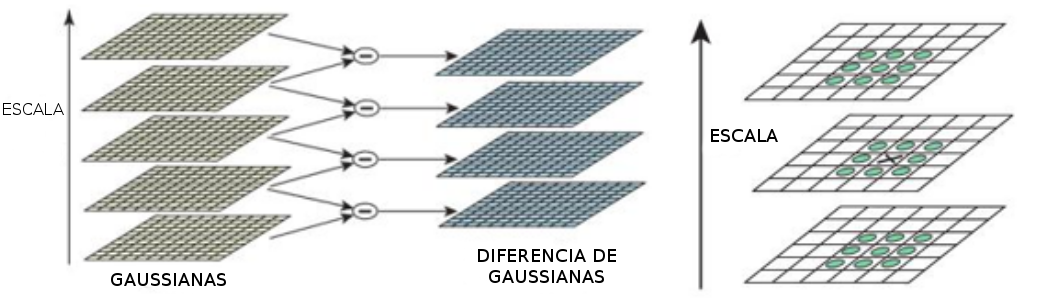
\includegraphics[width=0.85\textwidth]{sift-escalas}
	\caption[Detector SIFT]{Detección de máximos en el espacio de la escala DoG, adaptado de \cite{sift}}
	\label{imagen:sift-escalas}
\end{figure}

En segundo lugar para la localización de puntos de interés, se descartan los puntos encontrados en el paso anterior que no superen cierto valor de umbral, es decir, que no estén lo suficientemente contrastados con su entorno. Con esta etapa el algoritmo solo toma en cuenta los puntos claves mas fuertes por cada escala. Además, con el objetivo de eliminar los bordes suficientemente contrastados que no correspondan con esquinas, el algoritmo usa una matriz hessiana para calcular las curvaturas principales, y así quedarse solo con esquinas.

Para garantizar la invarianza con respecto a la rotación, se toman los píxeles vecinos al punto clave y se calcula la magnitud y dirección del gradiente en esa región. Con esto se hace un histograma de la magnitud del gradiente en cada dirección, donde el pico mayor del histograma indica la orientación. En el caso que exista un pico mayor al 80\% del pico principal, este se utiliza para crear otro punto de interés en la misma posición pero con la distinta rotación.

Finalmente para crear el vector descriptor por cada punto clave se crea una matriz de 16x16 alrededor de este, dividida en 4 subregiones de 4x4 píxeles con un histograma de orientaciones para cada uno. Seguidamente, el descriptor del punto será el vector con los valores de los histogramas de las regiones 4x4 concatenados. La figura \ref{imagen:descriptor} la representación del descriptor de SIFT.

\begin{figure}[H]
	\centering
	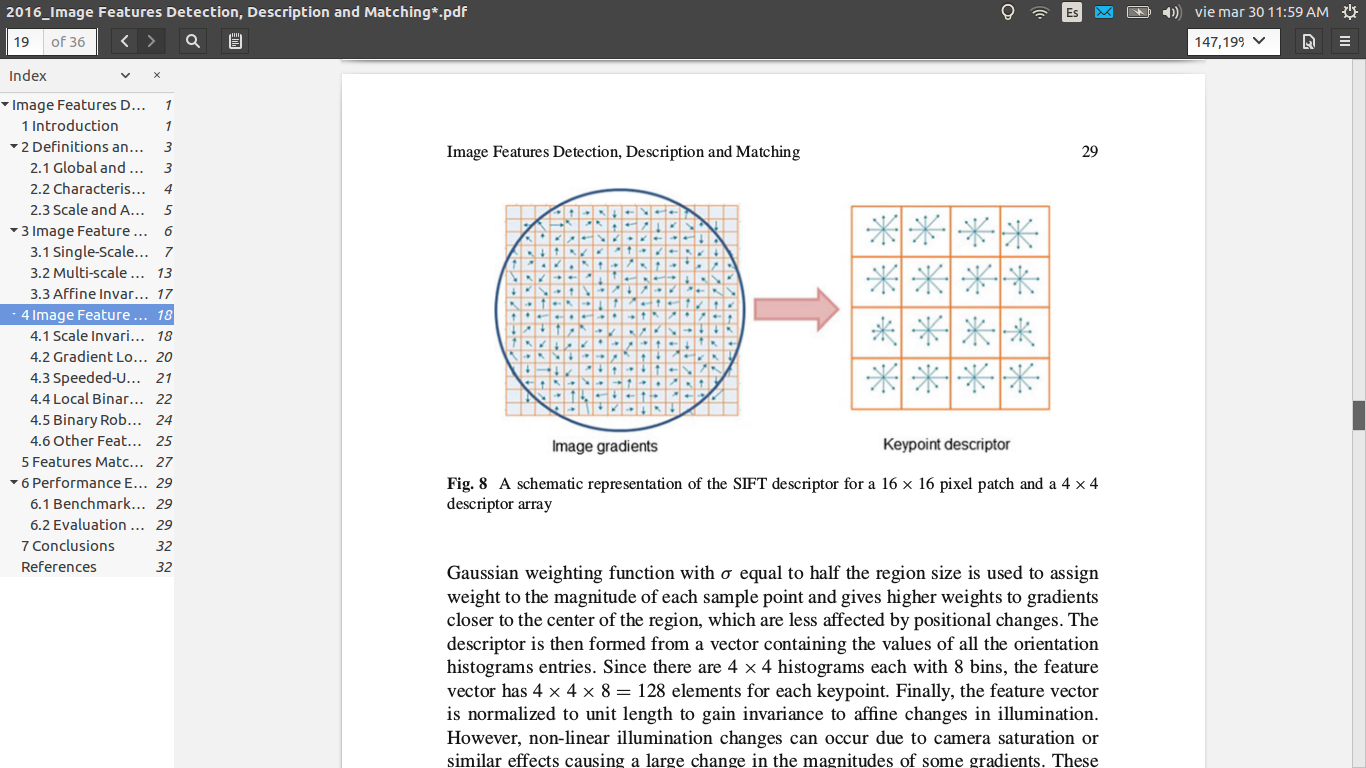
\includegraphics[width=0.7\textwidth]{sift-descriptor}
	\caption[Descriptor SIFT]{Izquierda: imagen de gradientes. Derecha: descriptor del punto clave. de \cite{sift}}
	\label{imagen:descriptor}
\end{figure}


En el año 2006, un grupo de tres  personas Bay, H., Tuytelaars, T. and Van Gool, L. desarrollan \textit{SURF} \cite{surf}, el cual es un detector y descriptor de características basado en SIFT, pero con modificaciones que aumentan su velocidad de detección. Si bien, sacrifica un poco de rendimiento y precisión, lo hace mas provechoso para aplicaciones embebidas que demanden mayor velocidad de computo y menor uso de recursos, como por ejemplo \textit{SLAM}. El proceso para la extracción de características por parte de este algoritmo se compone de los siguientes pasos:

Como primer paso, en lugar de aproximar el laplaciano de Gauss \textit{LoG} (del inglés: Laplacian of Gaussians) con la diferencia de Gaussianas (DoG) como lo hace SIFT, este algoritmo aproxima LoG con cuadrados para promediar la imagen. La ventaja de aplicar filtros con cuadrados es que con la ayuda de imágenes integrales el cálculo computacional se reduce en gran medida.

\begin{figure}[H]
	\centering
	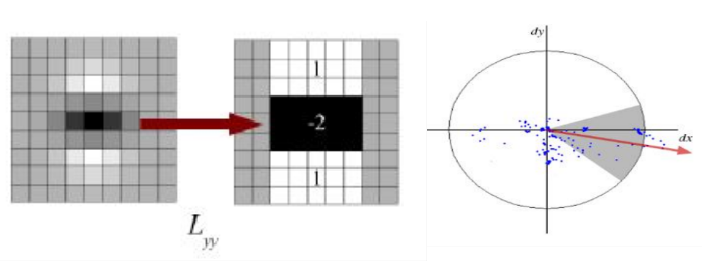
\includegraphics[width=0.8\textwidth]{surf}
	\caption[Detector y descriptor SURF]{Izquierda: aproximación a la derivada de segundo orden del filtro gaussiano (derivada parcial en el eje \textit{y}) y su aproximación con un filtro cuadrado. Derecha: vector de orientación del descriptor. Adaptado de \cite{surf}}
	\label{imagen:surf}
\end{figure}

En función de identificar la orientación, el algoritmo utiliza la respuesta wavelet Haar en horizontal y vertical en un vecindario de 6$s$ (donde $s$ es la escala evaluada) píxeles al rededor del punto de interés, Luego estas respuestas son representadas como puntos en el espacio, para luego calcular la orientación dominante con la suma de todos los resultados dentro de una ventana deslizante de apertura 60$^\circ$. En la figura \ref{imagen:surf} se puede visualizar en el lado izquierdo, la aproximación que realiza de la derivada de segundo orden del filtro gaussiano, y su aproximación con un filtro cuadrado. Del lado derecho se ilustra el vector de orientación en función a la distribución de puntos estudiados.

El siguiente avance importante en los algoritmos de detección aparece en el año 2011 con \textit{ORB} \cite{orb} (del inglés: Oriented FAST and Rotated BRIEF), este utiliza una combinación del detector FAST (del inglés: Features from Accelerated Segment Test) y del descriptor BRIEF (del inglés: Binary Robust Independent Elementary Features), este nuevo algoritmo esta caracterizado por su alta velocidad de procesamiento manteniendo un buen rendimiento, gracias al uso de un descriptor binario. 

Como se mencionó utiliza el algoritmo FAST, el cual consiste en encontrar esquinas evaluando los píxeles en un perímetro circular, de esta forma, un punto será detectado como esquina si la cantidad de píxeles de color opuesto al evaluado, supera cierto valor de umbral (ver izquierda en la figura \ref{imagen:orb}), posteriormente con el fin de aumentar la robustez, es aplicado el algoritmo de clasificación de esquinas de $Harris$. De igual forma se realiza con una estructura piramidal evaluando varias escalas (al igual que SIFT).

\begin{figure}[H]
	\centering
	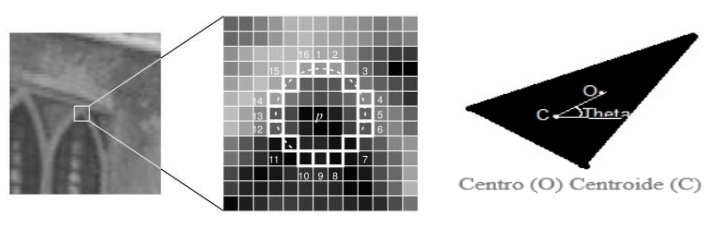
\includegraphics[width=0.9\textwidth]{orb}
	\caption[Detector y descriptor ORB]{izquierda: detección de esquinas usando FAST, de \cite{fast}. derecha: descriptor basado en BRIEF, adaptado de\protect\footnotemark }
	\label{imagen:orb}
\end{figure}

\footnotetext{\url{https://gilscvblog.com/2013/10/04/}}
Como el algoritmo FAST no toma en cuenta la orientación, en el ORB se modificó para que calculara la orientación de la siguiente forma: Se considera una región ubicada en el centro del punto estudiado, luego se calcula el centroide de la región en función a la intensidad de los puntos. De esta forma, la dirección del vector desde el punto central  hasta el centroide es asignado como vector de orientación. Observando a la derecha en \ref{imagen:orb} se aprecia un ejemplo del lugar del centroide \textit{(C)} y del centro \textit{(O)} para una región en particular.


Para el descriptor utiliza BRIEF, a diferencia de los anteriores (SIFT y SURF) este es un descriptor binario y no vectorial. El descriptor BFIEF produce una palabra de $n$-bits usando el algoritmo \textit{Local Binay Tests} (LBT), el problema de esta representación es que no es muy robusta ante cambios en la rotación. Para resolver esto ORB utiliza la información de la orientación previamente calculada en el paso de detección para aplicar LBT en esa orientación.

Los algoritmos de detección que se mencionaron hasta este momento tienen una característica en común, y es que cuando trabajan con el esquema piramidal lo hacen bajo el espacio de escala Gaussiano, el cual es una instancia particular de difusión lineal. De esta forma, al utilizar este filtro no se respetan los limites naturales de los objetos y se difumina del mismo nivel toda la región de la imagen cuando se avanza entre nieveles de escala.

Enfocándose en esta característica, en el año de \textit{2012} se desarrolla el detector y descriptor llamado KAZE \cite{kaze} por parte de \textit{Pablo Fernández Alcantarilla}. Este novedoso algoritmo opera completamente en un espacio de escala no lineal, y para ello utilizan un esquema de división de operadores aditivos (\textit{AOS}, del inglés: Additive Operator Splitting), que les permite obtener espacios de escala no lineales de forma eficiente. De este modo se puede realizar un difuminado localmente adaptativo, posibilitando que se remueva el ruido en las imágenes, manteniendo información importante sobre los bordes de los objetos al avanzar en el espacio de escala. En la figura \ref{imagen:kaze} se puede observar como afecta en los bordes de los objetos el aplicar un filtro de difusión lineal, y uno que no lo es, bajo el esquema propuesto por este algoritmo.

\begin{figure}[H]
	\centering
	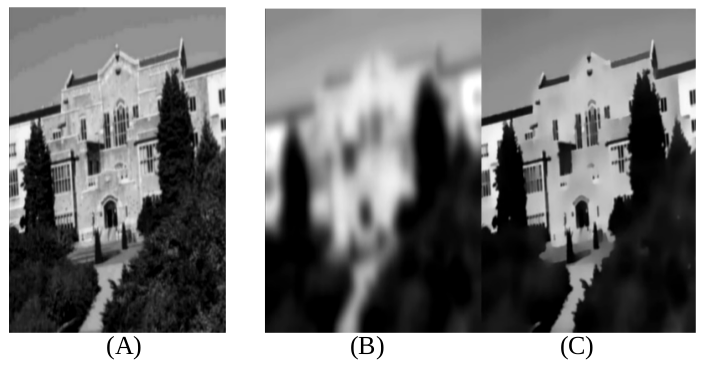
\includegraphics[width=0.85\textwidth]{kaze}
	\caption[Filtro no lineal propuesto por KAZE]{\textit{(A)}: imagen original, \textit{(B)} filtro lineal Gaussiano, \textit{(C)} filtro no lineal propuesto en KAZE, adaptada de \cite{kaze}}
	\label{imagen:kaze}
\end{figure}

Bajo este mismo esquema de difusión no lineal, el mismo autor en el año \textit{2013} desarrolla la versión acelerada de este algoritmo que recibe el nombre de \textit{A-KAZE} \cite{akaze} (del ingles: Accelerated KAZE). Esta mejora se utiliza un esquema basado en difusión explícita rápida \textit{FED} (del ingles: Fast Explicit Difussion) en lugar de \textit{AOS}, el cual es un nuevo esquema piramidal que incrementa en gran medida la velocidad de computo para construir el espacio de escala no lineal.

Para el calculo de la orientación el primer algoritmo \textit{KAZE} utiliza un descriptor para la orientación similar al que emplea SURF. Este encuentra la orientación dominante en un área circular de radio 6$s$ ($s$ corresponde con la escala), y para cada muestra del círculo se calcula la derivada de primer orden en las direcciones $X$ e $Y$, y se ponderan con una gaussiana centrada en el punto de interés. Luego, las respuestas de estas derivadas son representadas como puntos en un espacio vectorial, donde la orientación dominante se haya sumando las respuestas dentro de un segmento de circulo deslizante con apertura de 60$^\circ$.

Por otro lado, la versión acelerada \textit{A-KAZE} emplea un descriptor basado en una versión modificada del algoritmo de diferencia local binaria \textit{LDB} \cite{ldb} (del ingles: Local Difference Binary), llamado M-LBD (del ingles: Modified Local Difference Binary), el cual aprovecha al máximo la información del espacio de escala no lineal. La modificación consiste en hacer un sub-muestreo de cada región que divide la zona del descriptor, en lugar de calcular el promedio de todos los píxeles de la región, es decir, se tienen muestras de cada subdivisión para distintas escalas.


\subsection{Emparejadores de puntos característicos}

En este punto ya hemos estudiado los distintos algoritmos que permiten encontrar y clasificar puntos de interés en las imágenes. Ahora bien, es necesario identificar cuales de estos puntos corresponden con la misma ubicación, tal y como podemos observar en la figura \ref*{imagen:match}. Para establecer esta relación se utilizan los algoritmos emparejadores de características, los cuales relacionan estos puntos en base a los descriptores de dichos puntos.

\begin{figure}[H]
	\centering
	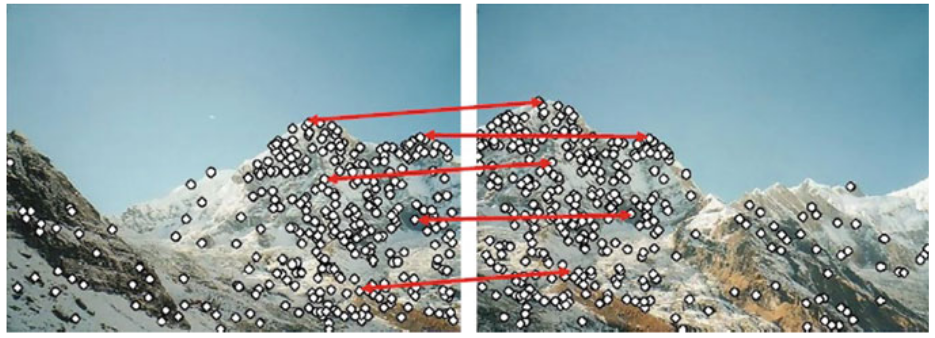
\includegraphics[width=14cm]{match}
	\caption[Emparejamiento de puntos característicos]{Emparejamiento de puntos que corresponden a la misma ubicación, de \cite{comp-vision} }
	\label{imagen:match}
\end{figure}

El proceso para realizar el emparejamiento consiste en el siguiente: Teniendo un punto característico $P_{1}$ perteneciente a la imagen $1$, y por otro lado se teniendo un punto $P_{2}$ perteneciente a la imagen $2$, Se calcula la distancia entre los descriptores $D_{1}$ y $D_{2}$. En el caso de descriptores vectoriales, esta distancia corresponde con la distancia \textit{Euclidiana}, dada por la siguiente expresión:
\begin{displaymath}
D = \sqrt{ (v_{1}-q_{1})^2 + (v_{2}-q_{2})^2 + \cdots + (v_{n}-q_{n})^2 }
\end{displaymath}
Donde $v_{n}$ corresponden con los componentes del vector descriptor $D1$, $q_{n}$ con los componentes del vector descriptor $D2$, y $n$ en el numero de componentes de ambos vectores. Por otro lado, para los descriptores binarios, se calcula la distancia \textit{Hamming}, dada por la siguiente expresión:
\begin{displaymath}
D = ||D_{1} \oplus D_{2}||
\end{displaymath}
Este proceso se repite hasta tener la distancia de cada punto de la imagen $1$ con todos los puntos de la imagen $2$, y viceversa. Al tener estas distancias, los puntos se emparejarán si y solo si se cumplen las siguientes condiciones: 

\begin{enumerate}[label=(\roman*)]
	\item El punto $P_{1}$ presenta la mejor distancia con $P_{2}$, en relación a todos los puntos de la imagen $2$.
	
	\item El punto $P_{2}$ presenta la mejor distancia con $P_{1}$ en relación a todos los puntos de la imagen $1$.
\end{enumerate}

Este proceso es mejor conocido como emparejamiento por fuerza bruta, ya que se compara entre todos los puntos por la mejor pareja posible. Si bien se asegura obtener el mejor emparejamiento, siendo viable para trabajar con pocos datos, el hecho de probar todas los casos posibles cuando se tiene una gran cantidad de puntos, incrementa en gran medida el tiempo de computo. Para efectuar este proceso de una forma eficiente se desarrollaron algoritmos basados en la búsqueda de vecinos mas cercanos. En este sentido se cuenta con el algoritmo \textit{kd-forest} (abreviado del inglés: k-dimensional forest), el cual es una mejora del algoritmo \textit{kd-tree} (abreviado del inglés: k-dimensional tree) para mejor desempeño al usar vectores multidimensionales, implementado en la librería para la rápida aproximación de vecinos mas cercanos FLANN \cite{flann} (del inglés: Fast Library for Approximate Nearest Neighbors).

%\textit{kd-tree} es una estructura de datos de segmentación de espacios para organizar puntos en un espacio de k dimensiones

\section{Módulo comparativo}

Una vez se conocen los algoritmos que se proponen utilizar, es necesario comparar su rendimiento bajo distintas condiciones, de modo que se pueda seleccionar el indicado para cada tipo de aplicación. En este sentido, se pretende estudiar el rendimiento en base a los siguientes parámetros:

\begin{itemize}
	\item \textbf{Tiempo de ejecución:} Tiempo en el que se detectan y describen las características en dos imágenes con las mismas dimensiones.
	
	\item \textbf{Cantidad de puntos detectados:} Cantidad total de puntos detectados en dos imágenes.
	
	\item \textbf{Cantidad de puntos emparejados:} Cantidad total de puntos emparejados correctamente luego de descartar parejas erróneas. 
\end{itemize}

Adicionalmente, se propone aplicar algunos métodos que permiten aumentar el rendimiento de los algoritmos de detección, así como también implementar un proceso que permita reducir o eliminar falsos positivos al emparejar puntos de interés. 

\subsection{Metodología}

El proceso planteado para la comparación, consiste en evaluar los parámetros antes mencionados para todas las combinaciones de extractores y emparejadores que se tienen, tal y como se ilustra en la figura \ref{imagen:comparacion}.

\begin{figure}[H]
	\centering
	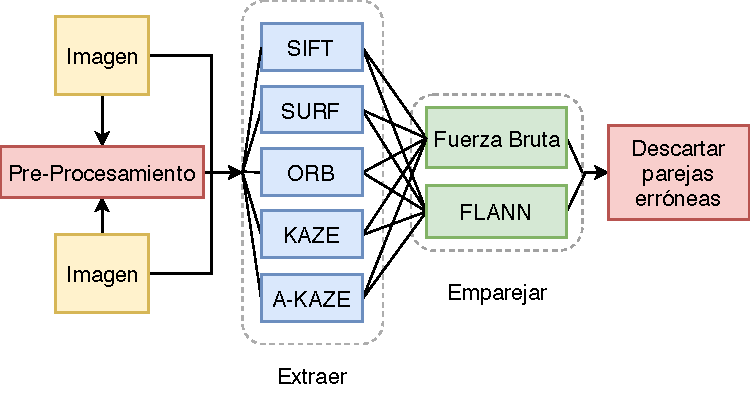
\includegraphics[width=14cm]{comparacion.pdf}
	\caption[Combinación de algoritmos para el analisis de rendimiento]{Combinaciones posibles del módulo comparativo}
	\label{imagen:comparacion}
\end{figure}

Cuando se utiliza un algoritmo para emparejar características, es muy común que existan parejas erróneas, puesto que al tener una gran cantidad de datos, varios pares de descriptores pueden tener la similitud necesaria para ser considerados como el mismo punto. Por esta razón es importante emplear una etapa que permita filtrar dichas parejas. Como ya se mencionó, se tienen distintos tipos de emparejadores, y en función a cada uno es necesario realizar el descarte de manera distinta. A continuación se describe el proceso en función a cada caso.

En el caso del algoritmo de fuerza bruta: Se obtiene la distancia de la mejor pareja, luego se descartan todas las pareas cuya distancia sea mayor que la mejor obtenida multiplicada por un factor de umbral. El proceso planteado se muestra en el algoritmo \ref{fuerzabruta}.

\begin{figure}[h]
	\centering
	\begin{minipage}{.7\linewidth}
		\begin{algorithm}[H] %or another one check
			\caption{Selección de buenas parejas - Fuerza bruta}
			\label{fuerzabruta}
			\SetAlgoLined
			$P{i}$ $\equiv$  $i$-ésima pareja\\
			$D_{i}$ $\equiv$ Distancia de la $i$-ésima pareja\\
			$N$ $\equiv$ Número de puntos emparejados\\
			$U$ $\equiv$ Umbral para descartar erróneos\\
			\Begin{
				$U = 0.8$\;
				\ForEach{i $\in$ n=1,2,$\cdots$,N}{
					\If{$D_{i} < mejorDistancia$}{
						$mejorDistancia = Dp_{i}$\;
					}
				}
				\ForEach{i $\in$ n=1,2,$\cdots$,N}{
					\If{$D_{i} > mejor distancia \cdot U$}{
						eliminar $P_{i}$\;
					}
				}
			}
		\end{algorithm}
	\end{minipage}
\end{figure}

En el caso del algoritmo bajo el esquema de vecinos mas cercanos: Se descarta cada pareja cuya distancia esté muy cercana a la distancia del vecino mas próximo. El proceso planteado se muestra en el algoritmo \ref{vecinosmascercanos}.

\begin{figure}[h]
	\centering
	\begin{minipage}{.75\linewidth}
		\begin{algorithm}[H] %or another one check
			\caption{Selección de buenas parejas - Vecinos mas cercanos}
			\label{vecinosmascercanos}
			\SetAlgoLined
			$P{i}$ $\equiv$ $i$-ésima pareja\\
			$D_{i}$ $\equiv$ Distancia de la $i$-ésima pareja\\
			$V_{i}$ $\equiv$ Distancia del vecino mas cercano de la $i$-ésima pareja\\
			$N$ $\equiv$ Número de puntos emparejados\\
			$U$ $\equiv$ Umbral para descartar erróneos\\
			\Begin{
				$U = 0.5$\;
				\ForEach{i $\in$ n=1,2,$\cdots$,N}{
					\If{$D_{i} > V_{i} \cdot U$}{
						eliminar $P_{i}$\;
					}
				}
			}
		\end{algorithm}
	\end{minipage}
\end{figure}

En segundo lugar, con el objetivo de mejorar la detección se implementa un proceso de pre-procesamiento en las imágenes de entrada. Tal y como se estudió en la sección teórica, para que un punto característico sea detectado, éste debe contener información que lo diferencie de su entorno cercano, en este caso esta diferencia es medida en función a su intensidad. En base a esta definición, se propone un algoritmo que permite mejorar el contraste en la imagen mediante la técnica de estirar su histograma. De esta forma cada imagen tendrá el máximo rango de excursión sobre las intensidades de sus puntos, permitiendo que los valores de umbral al detectar regiones, se superen con más facilidad.

Es importante destacar que para este proceso todas las imágenes fueron almacenadas usando variables de 8 bits, es decir, que cada valor es representado en un rango comprendido entre 0 y 255.

Para el calculo del histograma se obtiene la frecuencia de aparición de cada valor de intensidad en la imagen. Luego, se obtiene el valor de la intensidad para la cual, la cantidad de píxeles cuyo valor sea menor o igual a ésta, no supere el 1\% de la cantidad total de píxeles en la imagen, este punto es llamado percentil bajo. A continuación se repite este proceso par ubicar el percentil alto, el cual corresponde con la intensidad para la cual la cantidad de píxeles inferiores a ésta, no supera el 99\% de la cantidad total de píxeles. Al tener estos valores se aplican los siguientes criterios:

\begin{itemize}
	\item Todos los píxeles cuyo valor se encuentre por debajo del percentil bajo es igualado a 0.
	\item Todos los píxeles cuyo valor se encuentre por encima del percentil alto es igualado a 255.
	\item Todos los valores cuyo valor se encuentre entre el percentil bajo y el alto, es reescalado usando la siguiente ecuación: 
	\begin{displaymath}
		I_{pixel} = \frac{(I_{pixel} - P_{bajo}) \cdot 255}{P_{alto} - P_{bajo}}
	\end{displaymath}
\end{itemize}

En la figura \ref{imagen:stretch} se puede apreciar el cambio, tanto en el histograma como en la misma imagen, luego de aplicar el proceso previamente descrito.


\begin{figure}[h]
	\centering
	\vspace{0.6cm}
	\begin{tabular}{@{}cc@{}}
		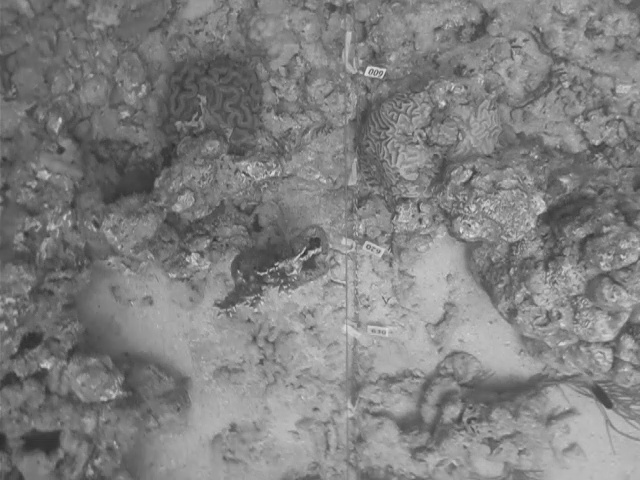
\includegraphics[width=.50\textwidth]{gray-01} &
		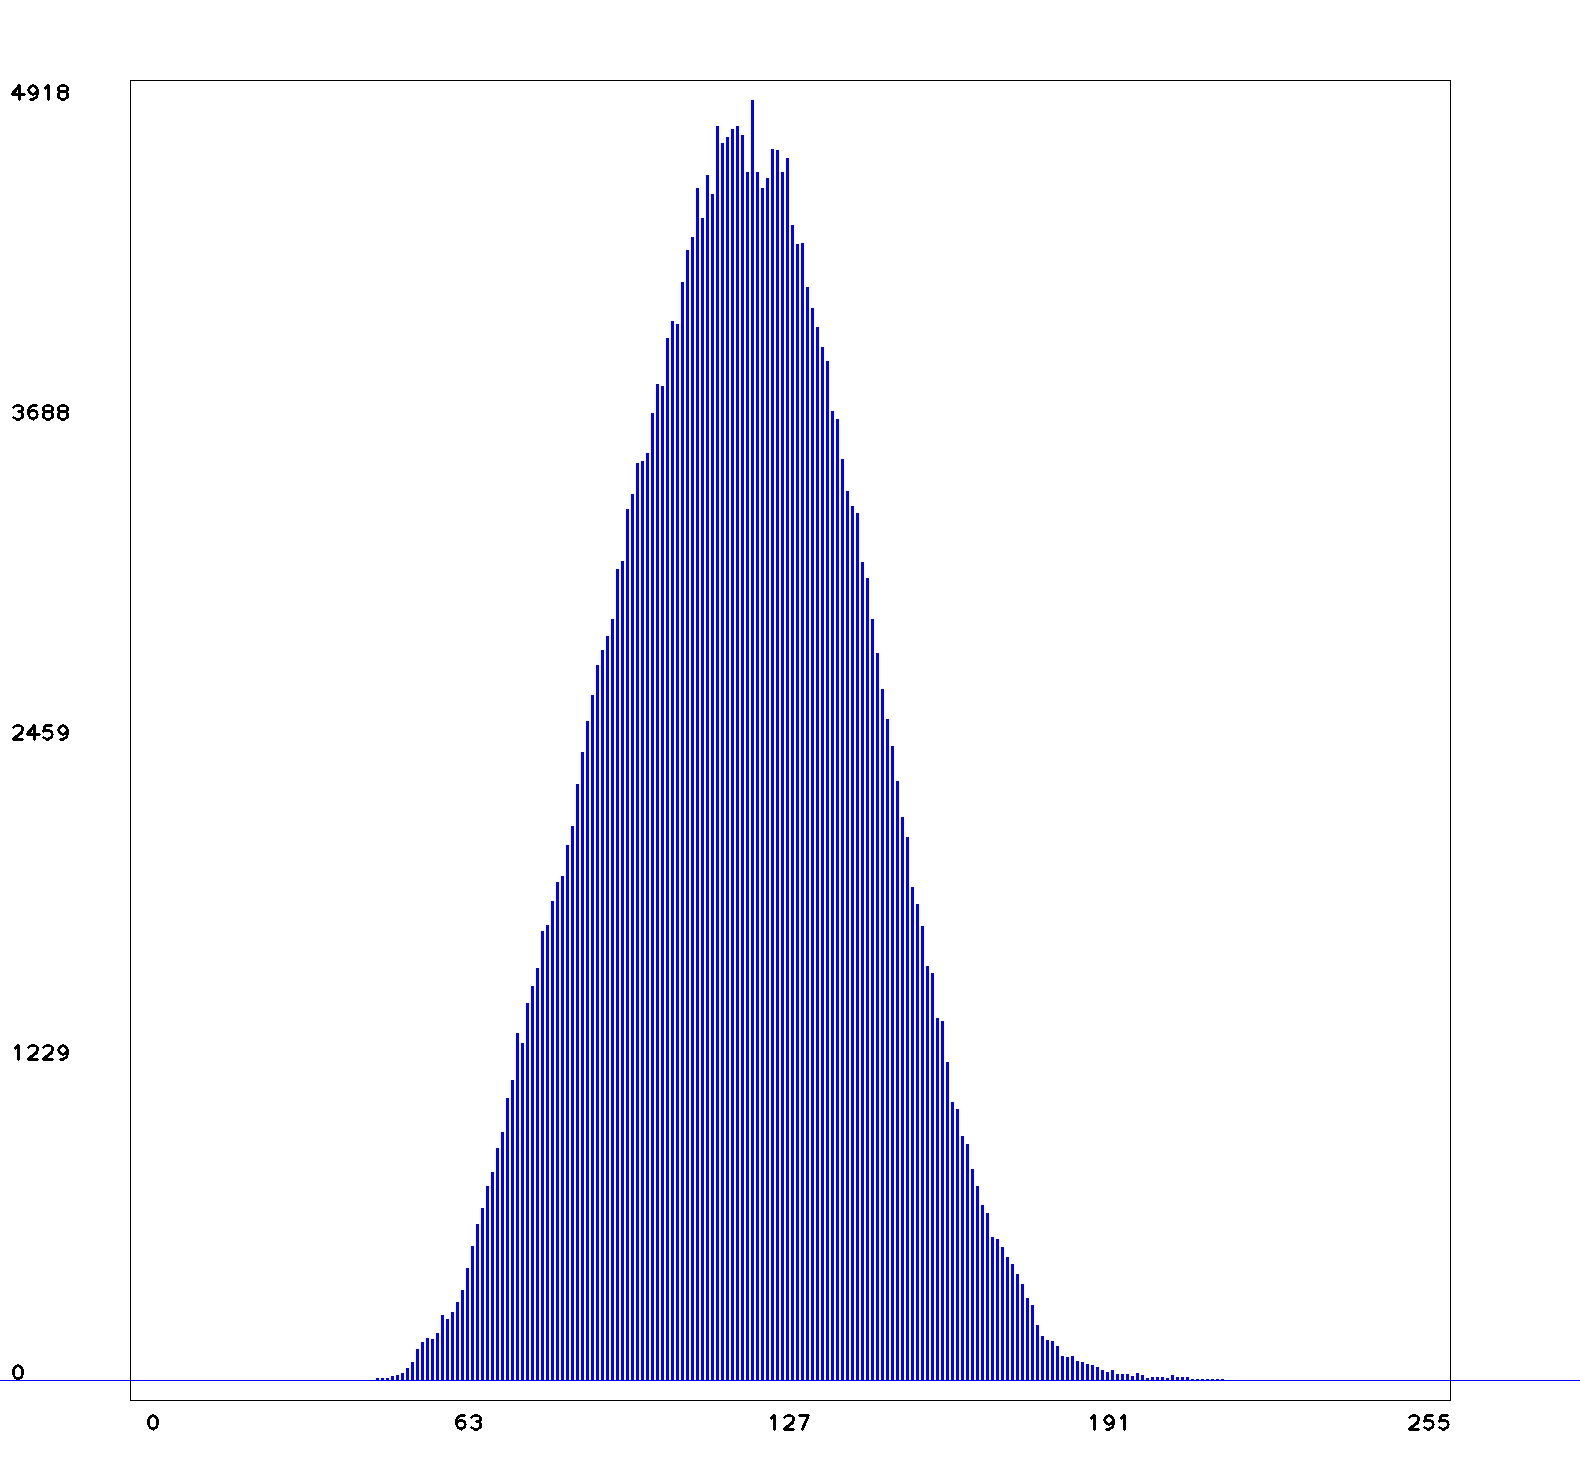
\includegraphics[width=.40\textwidth]{hist-01} \\
		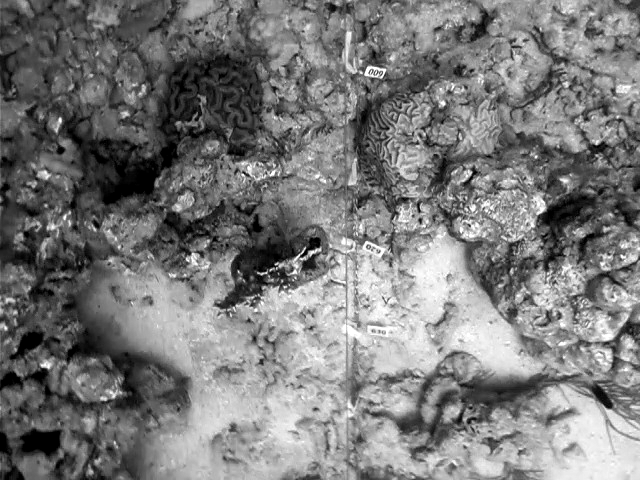
\includegraphics[width=.50\textwidth]{gray-stretch-01} &
		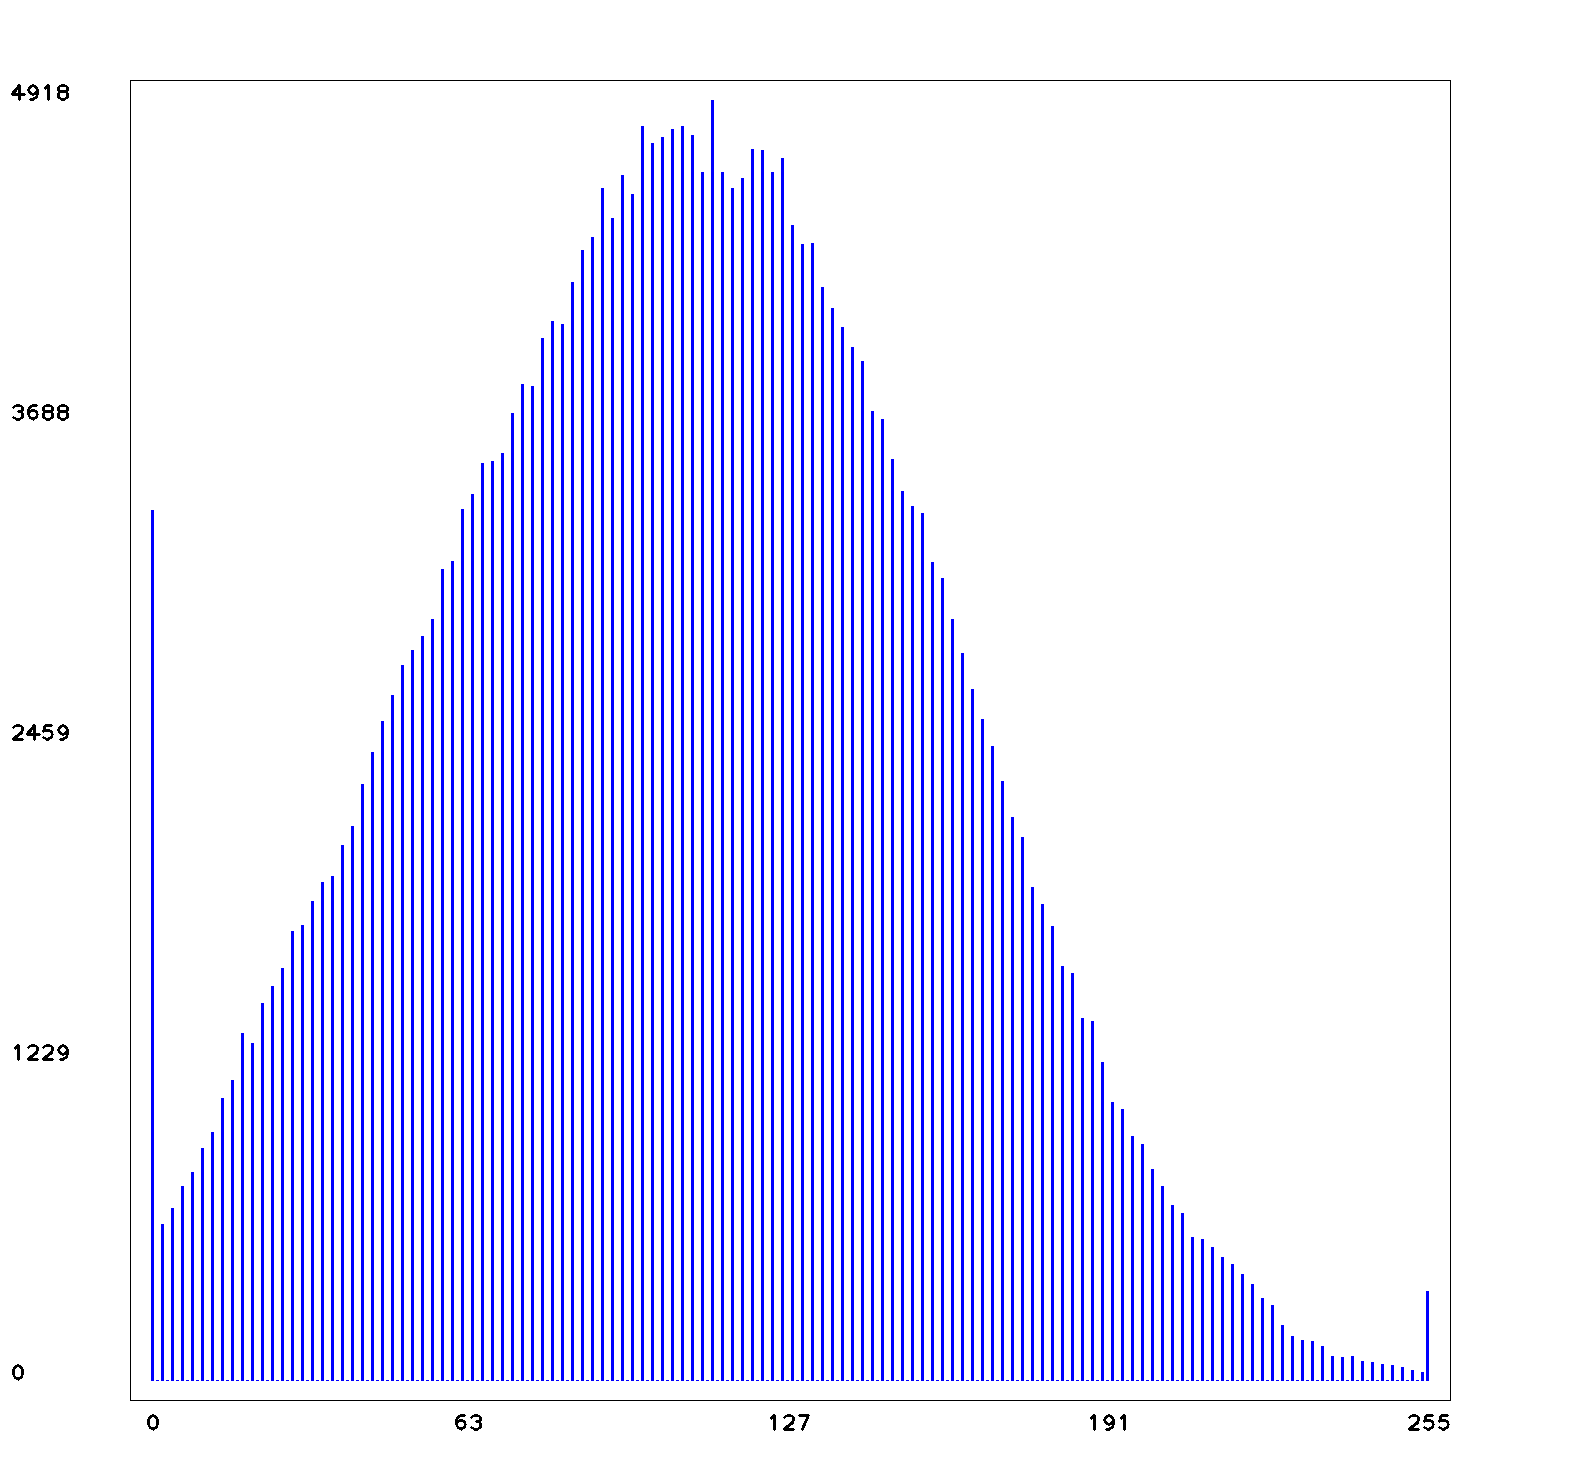
\includegraphics[width=.40\textwidth]{hist-stretch-01}
	\end{tabular}
	\captionof{figure}[Estiramiento del histograma]{Arriba: imagen original y su respectivo histograma a su derecha. Abajo: Imagen luego de aplicar el estiramiento del histograma, y su respectivo histograma a su derecha.}
	\label{imagen:stretch}
\end{figure}


%%%%%%%%%%%%%%%%%%%%%%%%%%%%%%%%%%%%%%%%%%%%%%%%%%%%%%%%%%%%%%%%%%%%%%%%%%%%%%%%%%%
\subsection{Resultados}

A continuación se presentan los resultados, para todas las combinaciones de extractores y emparejadores, bajo distintas condiciones de escena. Todas las pruebas mostradas en esta sección se realizaron utilizando un equipo con las siguientes características:  \textit{Intel\textsuperscript \textregistered } Core 2 Duo CPU E8400 @ 3.00Ghz.

En el cuadro \ref{0234} se observan los resultados para 61 pares de imágenes del fondo marino en la región de Chuspa (conjunto \textit{Chuspa}), ubicada en el estado Vargas, Venezuela. Adicionalmente, en la figura \ref{imagen:0234} se ilustran cuatro imágenes representativas del conjunto estudiado. Para esta prueba se utilizaron imágenes de $640\times480$ píxeles.

\begin{table}[h]
	\centering
	\captionof{table}{Comparación de rendimiento usando imágenes del conjunto \textit{Chuspa}}
	\label{0234}
	\renewcommand{\arraystretch}{0.8}% Tighter
	\begin{tabular}{@{}lllllll@{}}
		\toprule
			 &                				& SIFT 			& SURF & ORB 			& KAZE 				& A-KAZE \\ \midrule 
		       \hfill\vline& Total parejas  & \textbf{68679}& 32888&29637			& 6818 				& 6896   \\
		Fuerza Bruta \vline& Buenas parejas & 12601			& 3764 & 224 			& 1407 				& 520    \\
			   \hfill\vline& Precisión (\%) & 18.34			&11.44 &0.70 			&20.63 				& 7.54  \\
			   \vspace{0.3cm}
			   \hfill\vline& Tiempo (s)     & 38.27			&13.60 &\textbf{2.32}	&69.09 				& 16.99  \\
			   
			   \hfill\vline& Total parejas  & \textbf{68679}& 32888&29637			& 6818 				& 6896   \\
		FLANN  \hfill\vline& Buenas parejas &\textbf{13221} & 3895 & 282 			& 1416 				&553     \\ 
			   \hfill\vline& Precisión (\%) & 19.25			& 11.84& 0.95			& \textbf{20.76}	& 8.01 \\ 
			   \hfill\vline& Tiempo (s)     & 38.27			&13.60 &\textbf{2.32} 	&69.09 				& 16.99  \\
			   \bottomrule
	\end{tabular}
\end{table}


\begin{table}[h]
	\centering
	\captionof{table}{Comparación de rendimiento usando imágenes del conjunto \textit{Chuspa}, luego de aplicar estiramiento del histograma}
	\label{0234-2}
	\renewcommand{\arraystretch}{0.8}% Tighter
	\begin{tabular}{@{}lllllll@{}}
		\toprule
		&                				& SIFT 			& SURF & ORB 			& KAZE 				& A-KAZE \\ \midrule 
		\hfill\vline& Total parejas  & \textbf{235284}  & 98402&30500			& 59061 			& 62957   \\
		Fuerza Bruta \vline& Buenas parejas & 29200		& 7461 & 200 			& 11812 			& 3115    \\
		\hfill\vline& Precisión (\%) & 12.41			&7.58 &0.65 			&19.99 				& 4.94  \\
		\vspace{0.3cm}
		\hfill\vline& Tiempo (s)     & 113.29			&28.81 &\textbf{3.44}	&75.40 				& 21.66  \\
		
		\hfill\vline& Total parejas  & \textbf{235284}  & 98402&30500			& 59061 			& 62957   \\
		FLANN \hfill\vline& Buenas parejas &\textbf{31917}& 7461 & 257 			& 12522				& 3617     \\ 
		\hfill\vline& Precisión (\%) & 13.53			& 8.17& 0.84			& \textbf{21.20}	& 5.74 \\ 
		\hfill\vline& Tiempo (s)     & 63.81			&25.79 &\textbf{3.78} 	&75.20 				& 20.58  \\
		\bottomrule
	\end{tabular}
\end{table}

\begin{figure}[h]
	
	\centering
	\vspace{0.6cm}
	\begin{tabular}{@{}cccc@{}}
		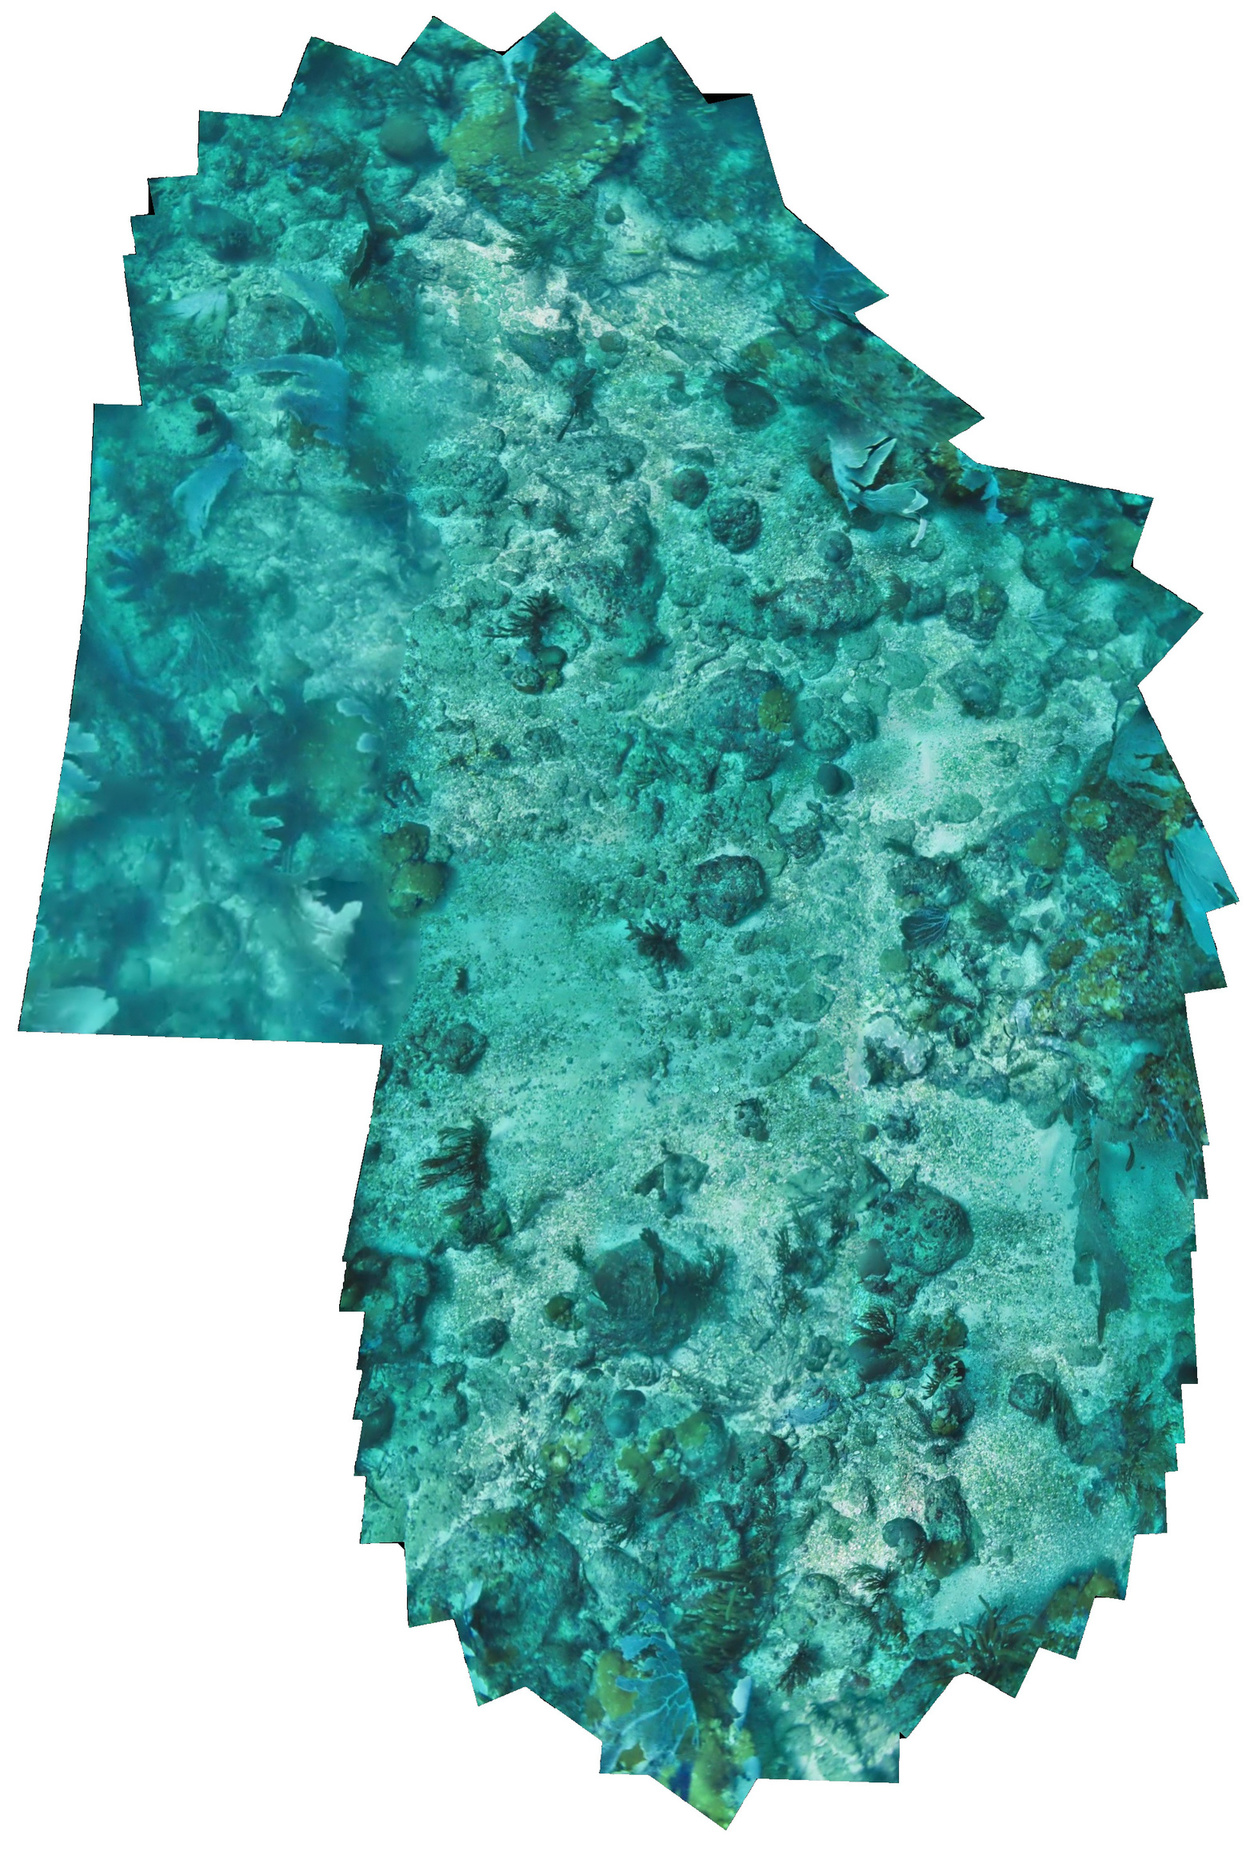
\includegraphics[width=.23\textwidth]{0234-1} &
		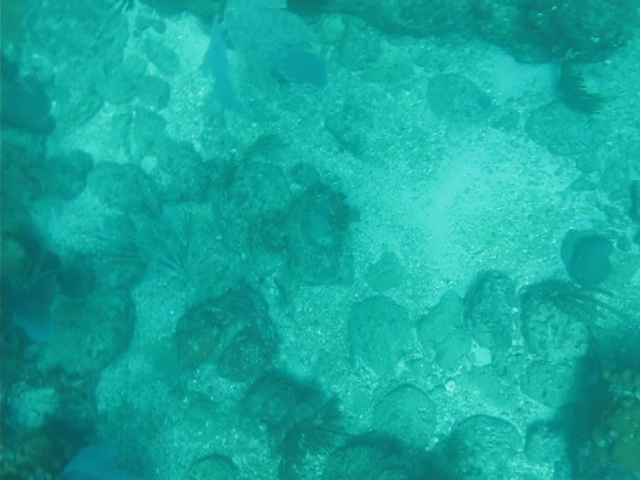
\includegraphics[width=.23\textwidth]{0234-2} &
		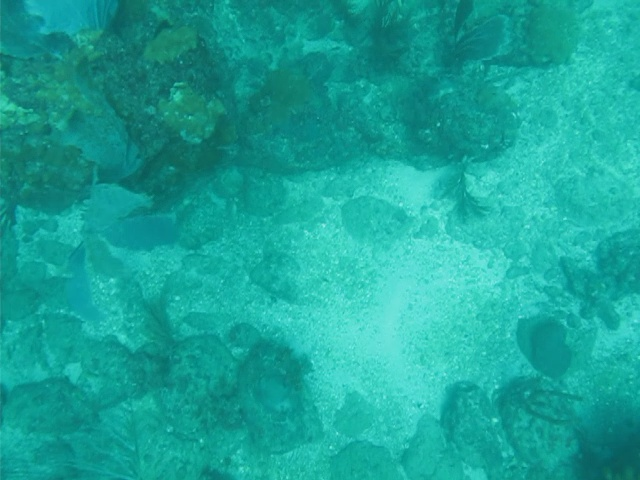
\includegraphics[width=.23\textwidth]{0234-3} &
		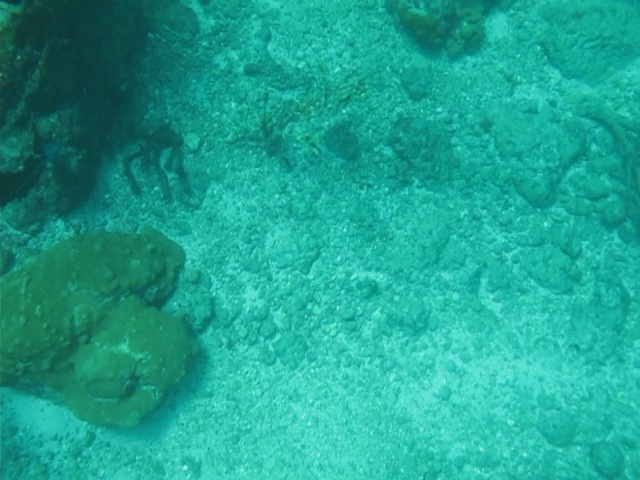
\includegraphics[width=.23\textwidth]{0234-4} 
	\end{tabular}
	\captionof{figure}{imágenes representativas del conjunto \textit{Chuspa}}
	\label{imagen:0234}
\end{figure}


En el cuadro \ref{SR} se observan los resultados para 42 pares de imágenes. Estas imágenes fueron proporcionadas por el centro Australiano de Robótica de Campo ACFR (del inglés: Australian Center for Field Robotics) y pertenecen al conjunto de datos \textit{ScottReef 25}. Adicionalmente, en la figura \ref{imagen:SR} se ilustran cuatro imágenes representativas del conjunto estudiado. Para esta prueba se utilizaron imágenes de $640\times480$ píxeles.

%\begin{figure}{\linewidth}
\begin{table}[h]
		\centering
		\captionof{table}{Comparación de rendimiento usando imágenes submarinas del conjunto \textit{ScottReef 25}}
		\label{SR}
		\renewcommand{\arraystretch}{0.8}% Tighter
		\begin{tabular}{@{}lllllll@{}}
			\toprule
			&              	 			& SIFT 			& SURF & ORB & KAZE & A-KAZE \\ \midrule 
			\hfill\vline& Total parejas  &\textbf{100620}&48955 &21000&17952 & 19430  \\
			Fuerza Bruta \vline& Buenas parejas & 3631 			& 1383 & 55  & 1511 & 239    \\
			\hfill\vline& Precisión (\%) & 3.60			&2.82  &0.26 & 8.41& 1.23  \\
			\vspace{0.3cm}
			\hfill\vline& Tiempo (s)     & 49.87& 16.97&\textbf{5.90} &52.74 & 15.05 \\
			
			\hfill\vline& Total parejas  &\textbf{100620}&48955 &21000			&17952 			& 19430  \\
			FLANN  \hfill\vline& Buenas parejas &\textbf{3987}  & 1480 & 65  			& 1604 			&282     \\ 
			\hfill\vline& Precisión (\%) & 3.96			&3.02  &0.30			& \textbf{8.93}& 1.45  \\
			\hfill\vline& Tiempo (s)     & 36.82			& 15.70& 5.95	& 51.48			& 15.22  \\ 
			\bottomrule
		\end{tabular}
\end{table}


\begin{table}[h]
	\centering
	\captionof{table}{Comparación de rendimiento usando imágenes submarinas del conjunto \textit{ScottReef 25}, luego de aplicar estiramiento del histograma}
	\label{SR-2}
	\renewcommand{\arraystretch}{0.8}% Tighter
	\begin{tabular}{@{}lllllll@{}}
		\toprule
		&              	 			& SIFT 			 & SURF & ORB & KAZE  & A-KAZE \\ \midrule 
		\hfill\vline& Total parejas  &\textbf{231242}&115193&21000&134065 & 127859  \\
		Fuerza Bruta \vline& Buenas parejas & 5987 	& 2317 & 62  & 7621 & 796    \\
		\hfill\vline& Precisión (\%) & 2.58			&2.01  &0.29 &5.68& 0.62  \\
		\vspace{0.3cm}
		\hfill\vline& Tiempo (s)     & 125.38& 36.427& 7.08 &78.11 & 35.47 \\
		
		\hfill\vline& Total parejas  		&\textbf{231242}		&115193 &21000	&134065 		& 127859  \\
		FLANN  \hfill\vline& Buenas parejas &\textbf{6847}  		& 2542  & 65  	& 9034 			&1052     \\ 
		\hfill\vline& Precisión (\%) 		& 2.96					&2.20   &0.30	& \textbf{6.73} & 0.82  \\
		\hfill\vline& Tiempo (s)     		& 60.10					&29.59 & \textbf{7.02}	& 66.69			& 26.72  \\ 
		\bottomrule
	\end{tabular}
\end{table}
	 
\begin{figure}[h]
 	\centering
 	\vspace{0.6cm}
 	\begin{tabular}{@{}cccc@{}}
 		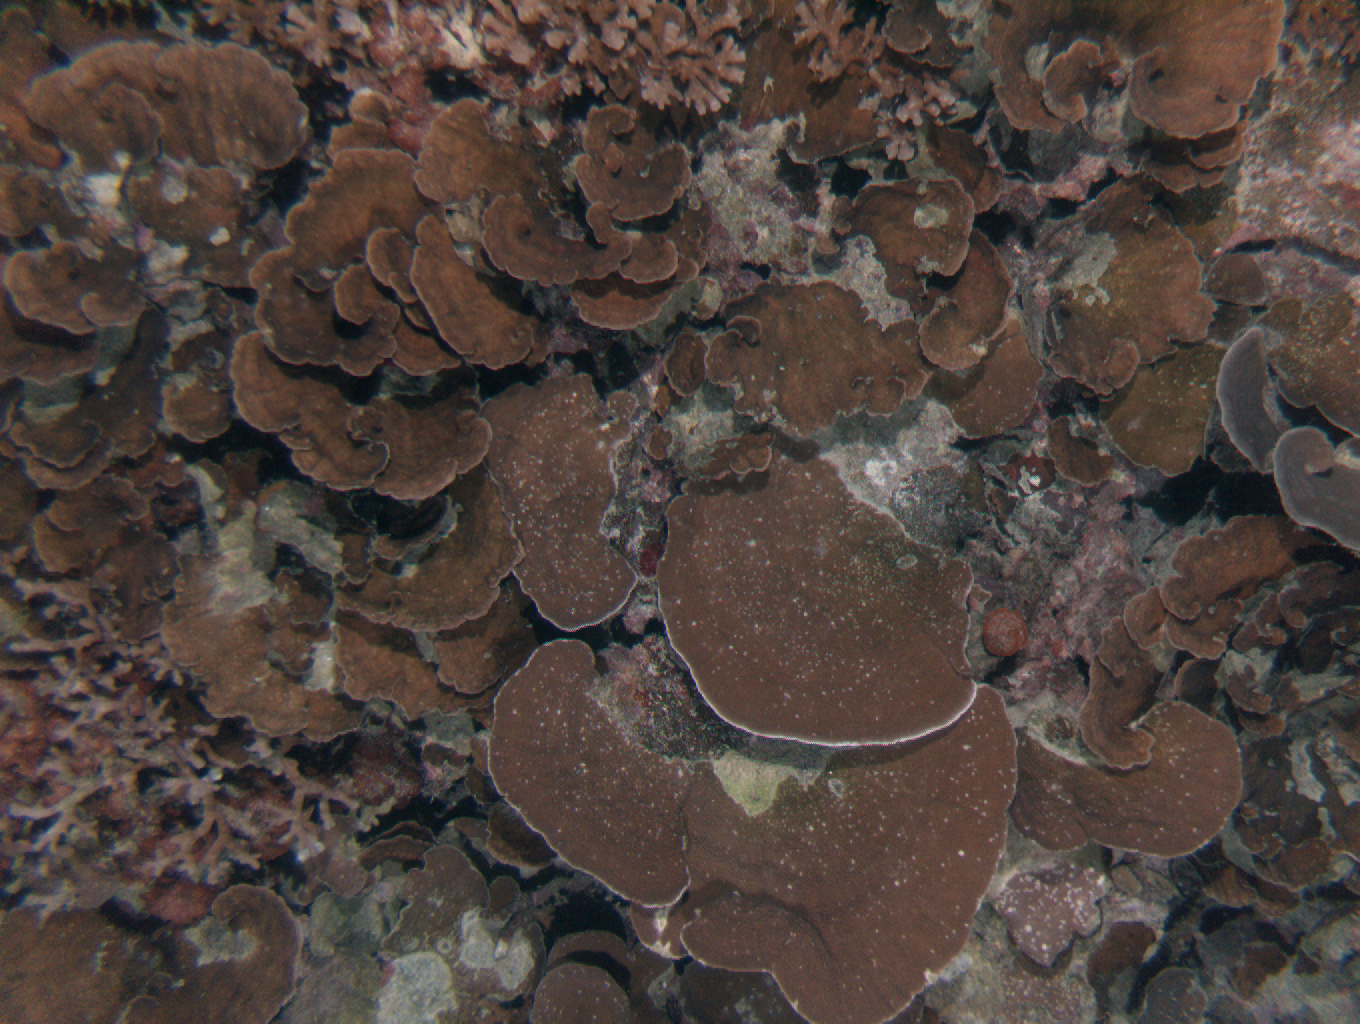
\includegraphics[width=.23\textwidth]{sr1} &
 		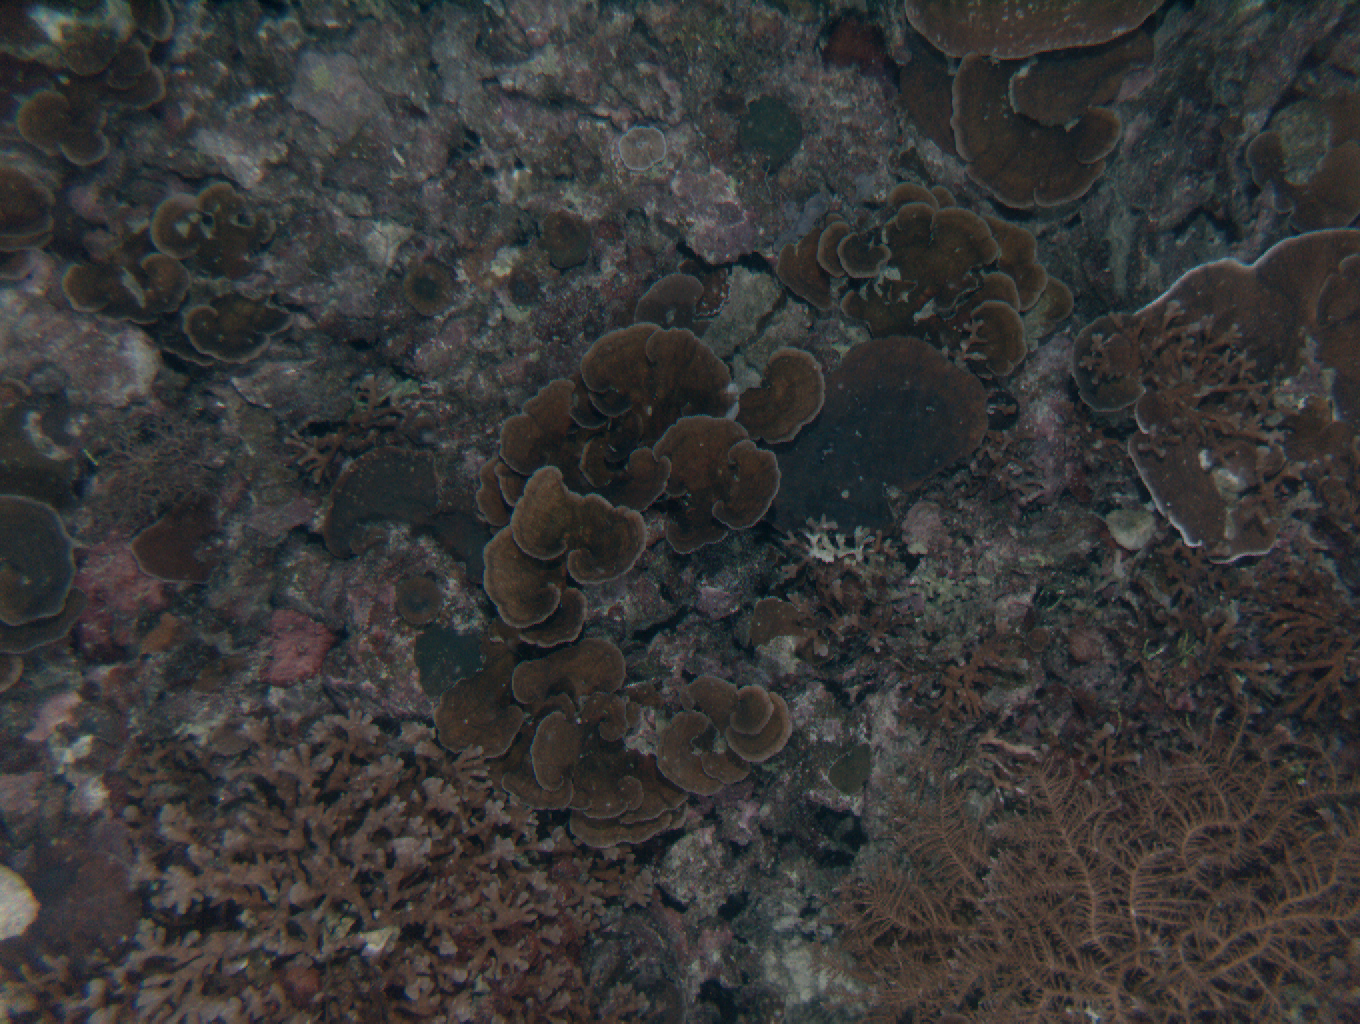
\includegraphics[width=.23\textwidth]{sr2} &
 		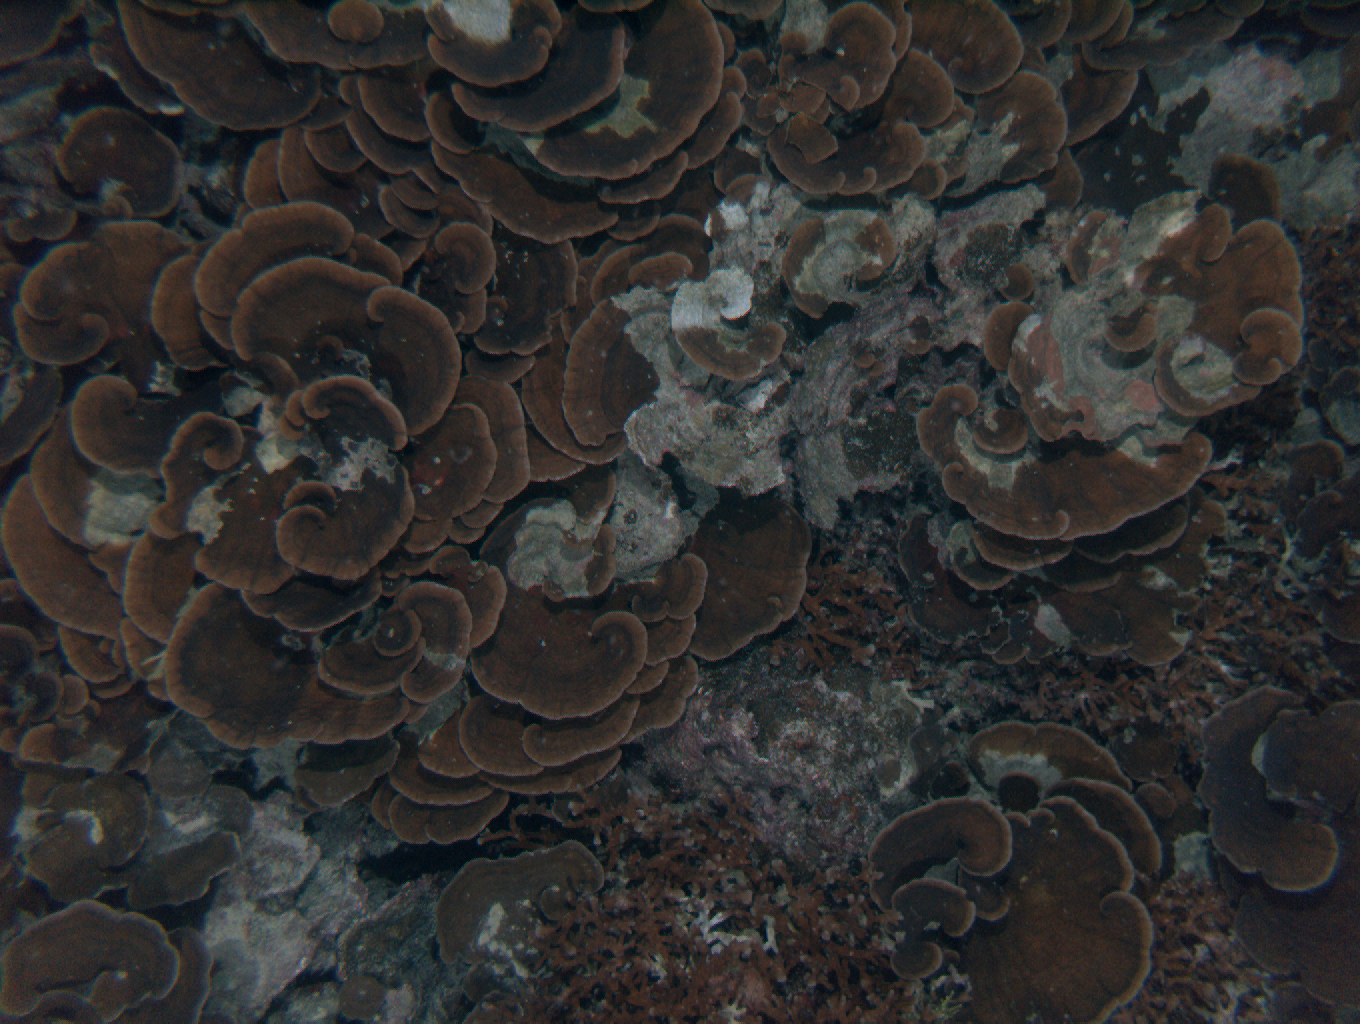
\includegraphics[width=.23\textwidth]{sr3} &
 		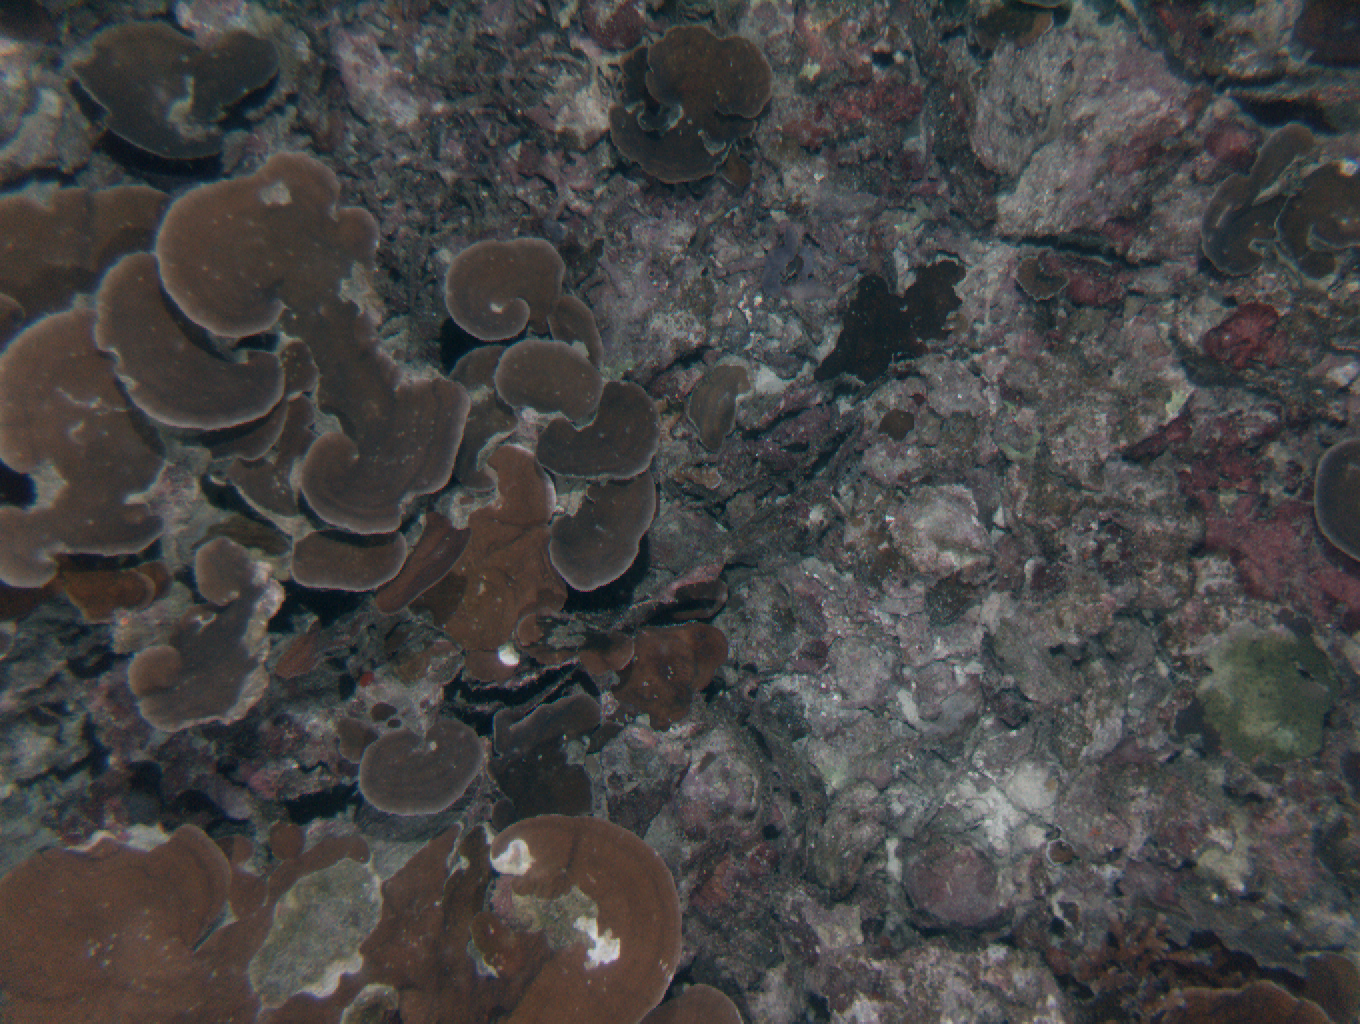
\includegraphics[width=.23\textwidth]{sr4} 
 	\end{tabular}
 	
 	\captionof{figure}{imágenes representativas del conjunto \textit{ScottReef 25}}
 	\label{imagen:SR}
 	
\end{figure}

En el cuadro \ref{0752} se observan los resultados para 51 pares de imágenes del fondo marino del parque nacional Mochima (conjunto \textit{Mochima}), ubicado en el estado Sucre, Venezuela. Adicionalmente, en la figura \ref{imagen:0234} se ilustran cuatro imágenes representativas del conjunto estudiado. Para esta prueba se utilizaron imágenes de $640\times480$ píxeles.

%\begin{figure}{\linewidth}
\begin{table}[h]
	\centering
	\captionof{table}{Comparación de rendimiento usando imágenes del conjunto \textit{Mochima}}
	\label{0752}
	\renewcommand{\arraystretch}{0.8}% Tighter
	\begin{tabular}{@{}lllllll@{}}
		\toprule
		&                      				& SIFT 			& SURF & ORB & KAZE & A-KAZE  \\ \midrule 
		\hfill\vline& Total parejas  &\textbf{116840}& 62472&25382&35934 & 34733   \\
		Fuerza Bruta \vline& Buenas parejas & 14659			& 6068 & 207 & 6760 & 1888    \\
		\hfill\vline& Precisión (\%) & 12.58			&9.71  &0.81 & 18.81 & 5.43  \\
		\vspace{0.3cm}
		\hfill\vline& Tiempo (s)     & 53.24			&18.37 & \textbf{2.30} &61.14 & 15.37   \\
		
		\hfill\vline& Total parejas  &\textbf{116840}& 62472&25382			&35934 				& 34733   \\
		FLANN  \hfill\vline& Buenas parejas &\textbf{15690} & 6426 & 242 			& 7175 				& 2136    \\
		\hfill\vline& Precisión (\%) & 13.42			& 5.48 &0.95  			& \textbf{19.96} 	& 6.14    \\ 
		\hfill\vline& Tiempo (s)     & 39.23			& 17.66& 2.44	& 62.07				& 15.07   \\ 
		\bottomrule
	\end{tabular}
\end{table}

\begin{table}[h]
	\centering
	\captionof{table}{Comparación de rendimiento usando imágenes del conjunto \textit{Mochima}, luego de aplicar estiramiento del histograma}
	\label{0752-2}
	\renewcommand{\arraystretch}{0.8}% Tighter
	\begin{tabular}{@{}lllllll@{}}
		\toprule
		&                      				& SIFT 			& SURF & ORB 		& KAZE 				& A-KAZE  \\ \midrule 
		\hfill\vline& Total parejas  &\textbf{146453}		& 75342&25440		&61107 				& 57797   \\
		Fuerza Bruta \vline& Buenas parejas & 16743			& 6879 & 208 		& 12105 			& 3310    \\
		\hfill\vline& Precisión (\%) & 11.43				&3.13  &0.81		& 19.80 			& 5.72  \\
		\vspace{0.3cm}
		\hfill\vline& Tiempo (s)     & 68.42				&22.05 & \textbf{2.80} &66.45       & 18.69   \\
		
		\hfill\vline& Total parejas  &\textbf{146453}& 75342&25440			&61107 				& 57797   \\
		FLANN  \hfill\vline& Buenas parejas &\textbf{18006} & 7328 & 244 			& 12890 			& 3773    \\
		\hfill\vline& Precisión (\%) & 12.29				& 9.72 &0.95  			& \textbf{21.09} 	& 6.52    \\ 
		\hfill\vline& Tiempo (s)     & 45.01				& 20.27& 2.88			& 64.77				& 17.57   \\ 
		\bottomrule
	\end{tabular}
\end{table}

\begin{figure}[h]
	\centering
	\vspace{0.6cm}
	\begin{tabular}{@{}cccc@{}}
		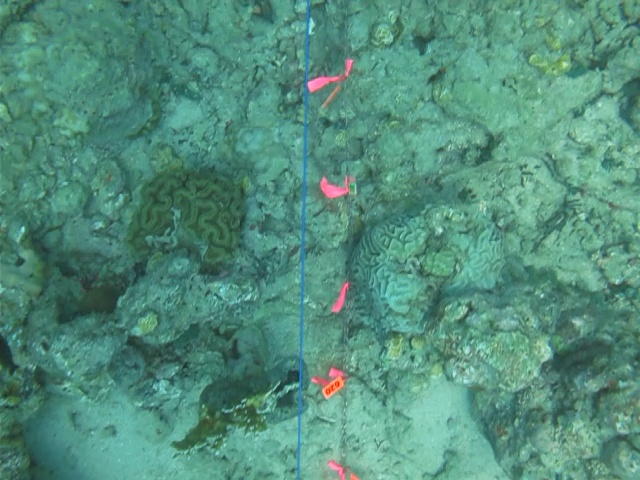
\includegraphics[width=.23\textwidth]{0752-1} &
		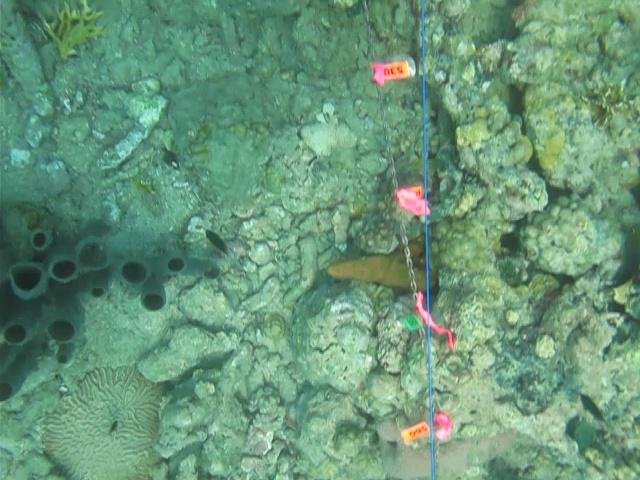
\includegraphics[width=.23\textwidth]{0752-2} &
		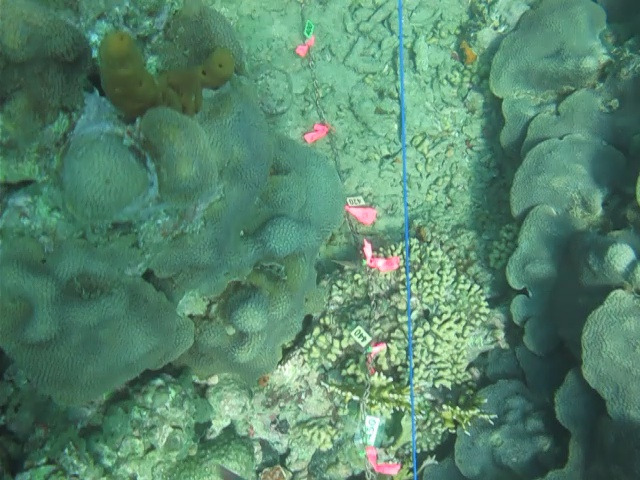
\includegraphics[width=.23\textwidth]{0752-3} &
		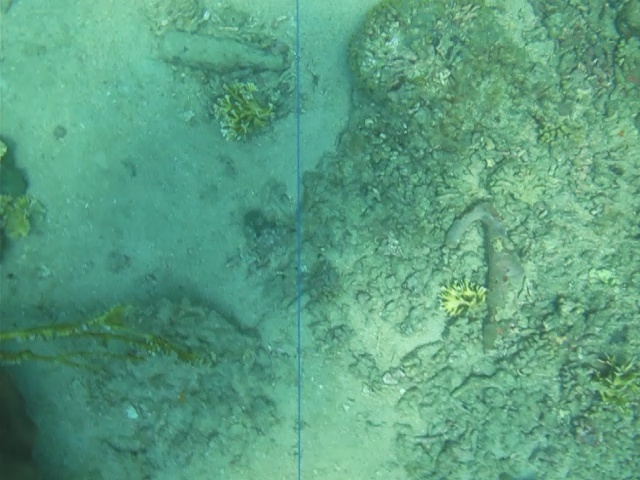
\includegraphics[width=.23\textwidth]{0752-4} 
	\end{tabular}
	\captionof{figure}{imágenes representativas del conjunto \textit{Mochima}}
	\label{imagen:0752}
\end{figure}

En el cuadro \ref{geotagg} se observan los resultados para 50 pares de imágenes aéreas de una cantera de grava (conjunto \textit{Grava}), ubicado en Suiza. Estas imágenes fueron proporcionadas por la empresa SenseFly\footnote{\url{https://www.sensefly.com/education/datasets/}} y capturadas por un dron eBee\footnote{\url{https://www.sensefly.com/drone/ebee-mapping-drone/}}.  Adicionalmente, en la figura \ref{imagen:geotag} se ilustran cuatro imágenes representativas del conjunto estudiado. Para esta prueba se utilizaron imágenes de $1280\times960$ píxeles.

\begin{table}[h]
	\centering
	\caption{Comparación de rendimiento usando imágenes del conjunto \textit{Grava}}
	\label{geotagg}
	\begin{tabular}{@{}lllllll@{}}
		\toprule
		&                      				& SIFT 			& SURF & ORB & KAZE  & A-KAZE  \\ \midrule 
			   \hfill\vline& Total parejas  &\textbf{336189}& 222251&25000&108819& 121914   \\
		Fuerza Bruta \vline& Buenas parejas & 21006			& 5853 & 126 & 10290 & 3240  \\
			   \hfill\vline& Precisión (\%) & 3.24			&2.63  & 0.5   & 9.45& 2.65  \\
				\vspace{0.3cm}
			   \hfill\vline& Tiempo (s)     & 282.76		&116.38 & 28.84 &309.29 & 92.71   \\
		
			   \hfill\vline& Total parejas  &\textbf{336189}& 222251&25000			&108819				& 121914   \\
		FLANN  \hfill\vline& Buenas parejas &\textbf{22610} & 6525 & 143			& 10861				& 3749    \\
			   \hfill\vline& Precisión (\%) & 6.72			& 2.93 &0.57  			& \textbf{9.98} 	& 3.07    \\ 
			   \hfill\vline& Tiempo (s)     & 153.12		& 90.27& \textbf{28.53}	& 299.59			& 81.52   \\ 
		\bottomrule
	\end{tabular}
\end{table}
\begin{table}[h]
	\centering
	\caption{Comparación de rendimiento usando imágenes del conjunto \textit{Grava}, luego de aplicar estiramiento del histograma}
	\label{geotagg-2}
	\begin{tabular}{@{}lllllll@{}}
		\toprule
		&                      				& SIFT 			& SURF & ORB & KAZE  & A-KAZE  \\ \midrule 
		\hfill\vline& Total parejas  &\textbf{335418}		& 221287&25000&108124& 121122   \\
		Fuerza Bruta \vline& Buenas parejas & 20943			& 5812 & 127 & 10313 & 3239  \\
		\hfill\vline& Precisión (\%) & 6.24			&2.62  & 0.58  & 9.53& 2.67  \\
		\vspace{0.3cm}
		\hfill\vline& Tiempo (s)     & 278.97		&114.86 & 29.54 &300.12 & 92.31   \\
		
		\hfill\vline& Total parejas  &\textbf{335418}& 221287&25000			&108124				& 121122   \\
		FLANN  \hfill\vline& Buenas parejas &\textbf{22555} & 6509 & 149	& 10880				& 3754    \\
		\hfill\vline& Precisión (\%) & 6.72			& 2.94 &0.59  			& \textbf{10.06} 	& 3.09   \\ 
		\hfill\vline& Tiempo (s)     & 153.71		& 88.25& \textbf{29.44}	& 294.61			& 83.68   \\ 
		\bottomrule
	\end{tabular}
\end{table}

\begin{figure}[h]
	\centering
	\begin{tabular}{@{}cccc@{}}
		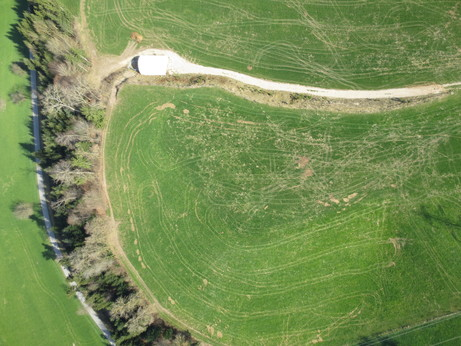
\includegraphics[width=.23\textwidth]{geotagg-1} &
		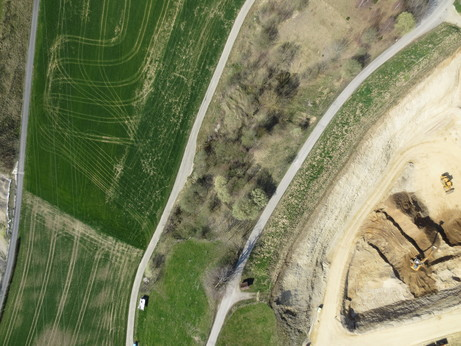
\includegraphics[width=.23\textwidth]{geotagg-2} &
		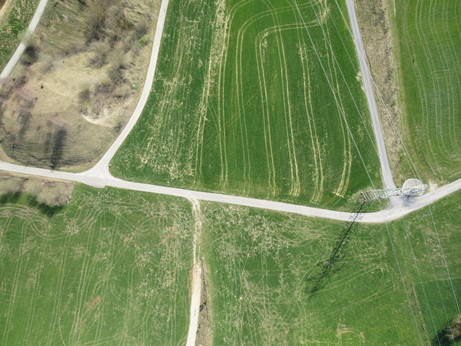
\includegraphics[width=.23\textwidth]{geotagg-3} &
		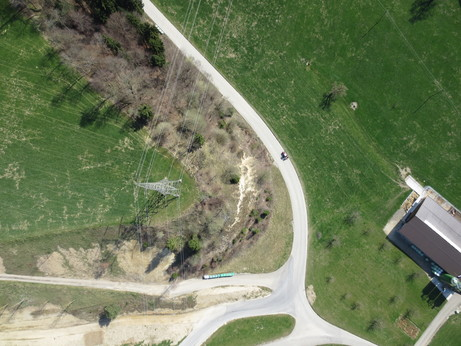
\includegraphics[width=.23\textwidth]{geotagg-4} 
	\end{tabular}
	\caption{imágenes representativas del conjunto \textit{Grava}}
	\label{imagen:geotag}
\end{figure}

Presentadas las pruebas, analizaremos el rendimiento de todas las combinaciones estudiadas en función a los parámetros descritos al inicio de la sección.

Es evidente la inversa relación entre la cantidad de puntos detectados y el tiempo que le toma ese proceso. En función a la detección, podemos acotar que los algoritmos SIFT y KAZE presentan la mayor cantidad de parejas correctas, siendo SIFT el que permanece con el mayor numero a lo largo de todas las pruebas. Este resultado está relacionado con el uso de descriptores vectoriales, que permiten una descripción mas robusta de los puntos detectados. Además que en el caso de SIFT no se realiza ninguna aproximación para la obtención de las diferentes escalas de la imagen.

Por el contrario, Aquellos algoritmos que utilizan descriptores binarios presentan un menor rendimiento en base a parejas emparejadas. Sin embargo, esta característica les permite realizar la extracción con una velocidad mucho mayor, siendo este un patrón que se mantiene a lo largo de todas las pruebas.

Analizando los resultados del extractor \textit{KAZE}, Si bien no ofrece la mayor cantidad de parejas correctas, presenta el mejor cociente entre parejas totales y correctas. Lo que indica un gran nivel de robustez en su descriptor, ya que un alto porcentaje de las parejas encontradas en un principio, efectivamente corresponden con el mismo punto.

Comparando el rendimiento de los emparejadores, podemos observar que para la mayoría de los casos el algoritmo FLANN aumenta la cantidad de parejas correctas, y al mismo tiempo disminuye el tiempo computacional. Si bien para la mayoría de las pruebas no se tiene un mejora significativa en términos de tiempo, es debido a que este algoritmo ofrece mayores beneficios cuando la cantidad de parejas a estudiar es mucho mas elevada. Este punto se evidencia mayormente en los resultados del algoritmo SIFT, el cual ofrece mayor cantidad de parejas, y por lo tanto mayor conjunto de puntos a emparejar.

Por ultimo podemos destacar el importante aumento en la cantidad de parejas detectadas, para los casos en los que se aplicó el pre-procesamiento en la entrada. Como ya se mencionó, se debe al aumento en el contraste, lo que produce que la diferencia entre un punto característico y su vecindario se incremente, aumentando al mismo tiempo la posibilidad de ser detectado y luego emparejado.

% Intel Core 2 Duo CPU E8400 @ 3.00 Ghz
% 3.7 GiB RAM

\section{Resumen}

El proceso de establecer la relación entre las imágenes, es un paso muy importante en la etapa de registro. De esta forma, la selección del algoritmo para la extracción de características, así como también la técnica que se use para establecer las correspondencias determinará la calidad final del mapa. Tal y como se presentó, se dispone de una gran cantidad de algoritmos para la extracción de características locales, así como también métodos eficientes para emparejarlos. Esta diversidad permite que se cuente con algoritmos que se comporten de manera eficiente para cada tipo de aplicación, o en el caso de mapeo, para cada tipo de escena. 

En el presente capítulo se logró establecer una clasificación sobre los algoritmos de generación, en función a como aborden las etapas mas importantes de éste. Tomando en cuenta los distintos métodos y técnicas, se planteó un sistema que combina aquellas que presentan los mejores resultados, considerando los requerimientos del presente proyecto. Al mismo tiempo se describió el funcionamiento de todos algoritmos que se plantean implementar en el sistema, permitiendo que se puedan plantear técnicas para mejorar el rendimiento en la extracción y emparejamiento. 

Tras los resultados mostrados, se logró evidenciar claramente el rendimiento de cada combinación en función a los parámetros de tiempo y cantidad de parejas. Lo que permite una selección en función de los requerimientos de la aplicación, y debido a la modularidad del esquema planteado es posible reemplazar cualquiera de los algoritmo presentes para extraer y emparejar sin afectar el resto del proceso para la construcción del mosaico.